\section{MultiFold technical closure}
\label{sec:multifoldtechnicalclosure}

The remaining 11 observables not shown in Sec.~\ref{sec:technicalclosure:multifold} are shown in Fig.~\ref{fig:technicalclosureMulti:mass2},~\ref{fig:technicalclosureMulti:ntracksjet2},~\ref{fig:technicalclosureMulti:pT_trackj2},~\ref{fig:technicalclosureMulti:tau1_trackj2}, and~\ref{fig:technicalclosureMulti:y_trackj2},~\ref{fig:technicalclosureMulti:tau2_trackj1},~\ref{fig:technicalclosureMulti:tau2_trackj2},~\ref{fig:technicalclosureMulti:tau3_trackj1},~\ref{fig:technicalclosureMulti:tau3_trackj2},~\ref{fig:technicalclosureMulti:yll},~\ref{fig:technicalclosureMulti:ptll}.

\begin{figure}[h!]
\centering
\subfloat[Input histograms]{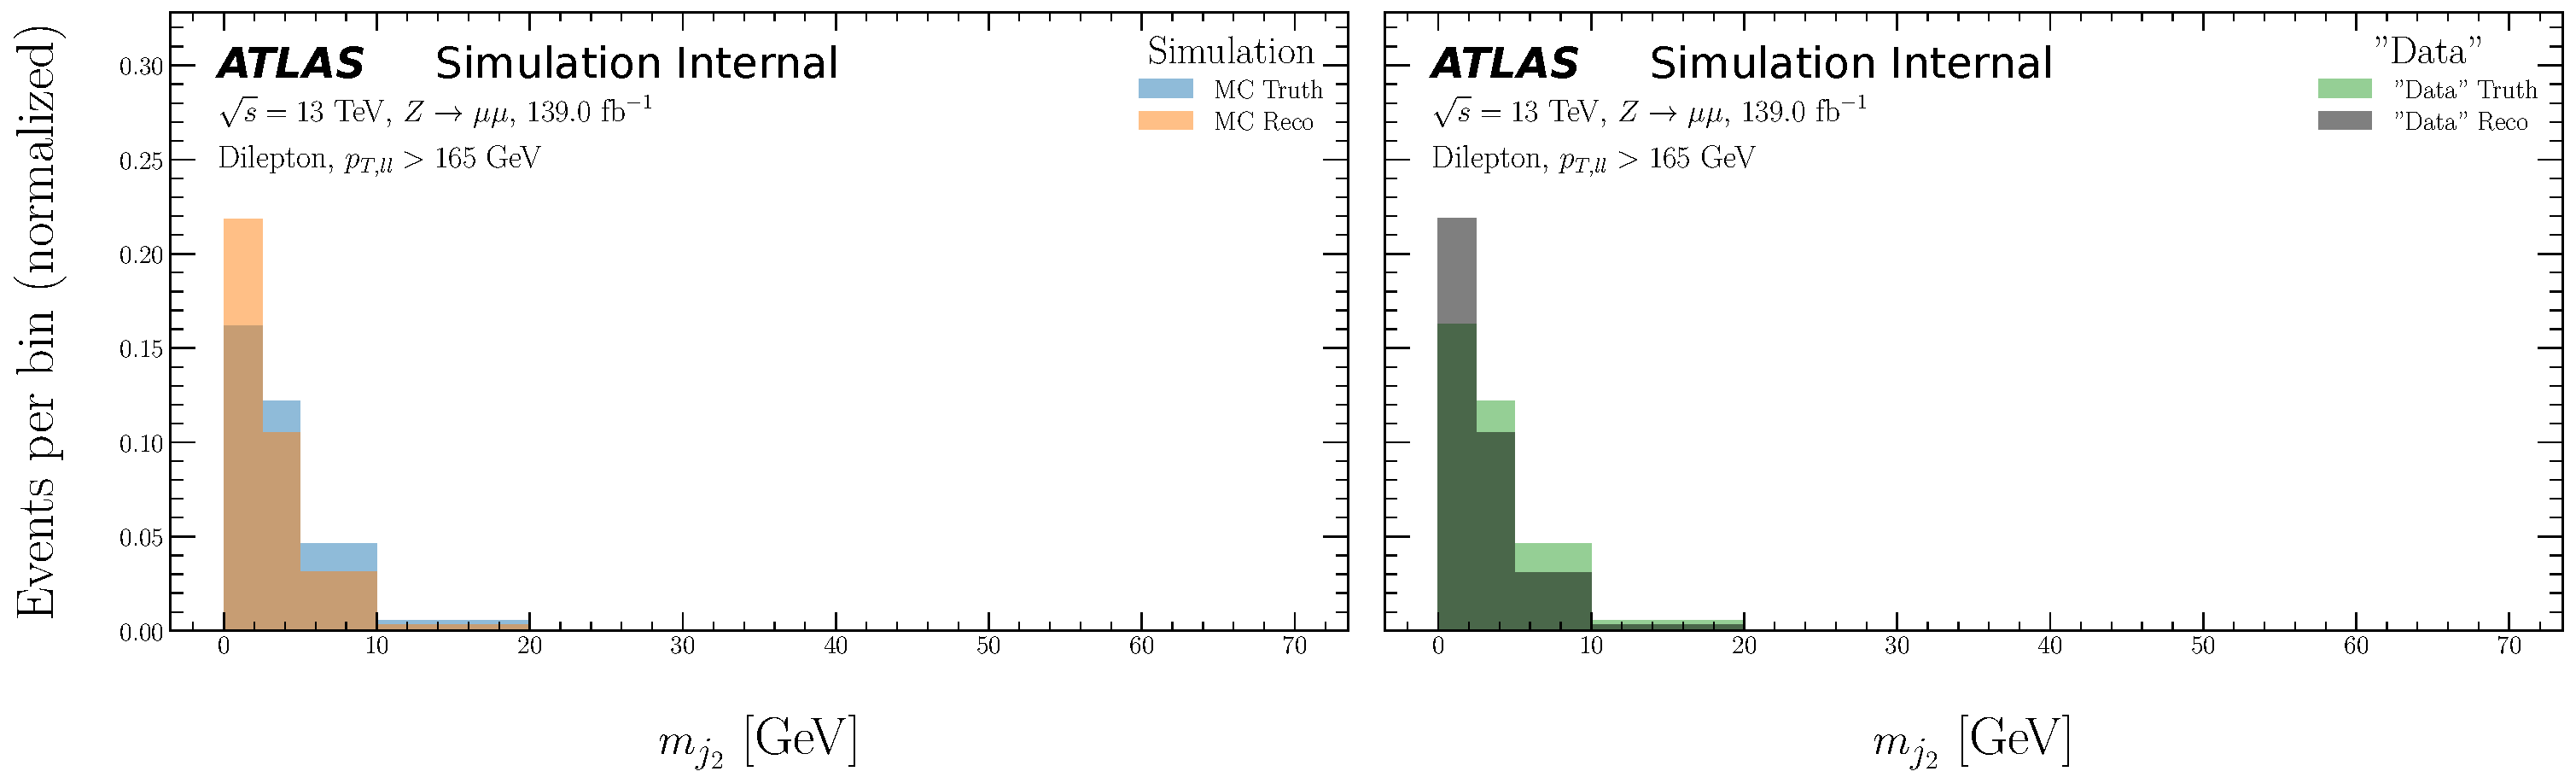
\includegraphics[width=0.95\textwidth]{figures/ATLASOmniFold-StressTest/ATLASOmniFold-TechnicalClosureTest/MultiFold/m_trackj2/ATLASOmniFold-TechnicalClosureTest-MultiFold-m_trackj2-Distributions.pdf}}\\
\subfloat[After 1 iteration]{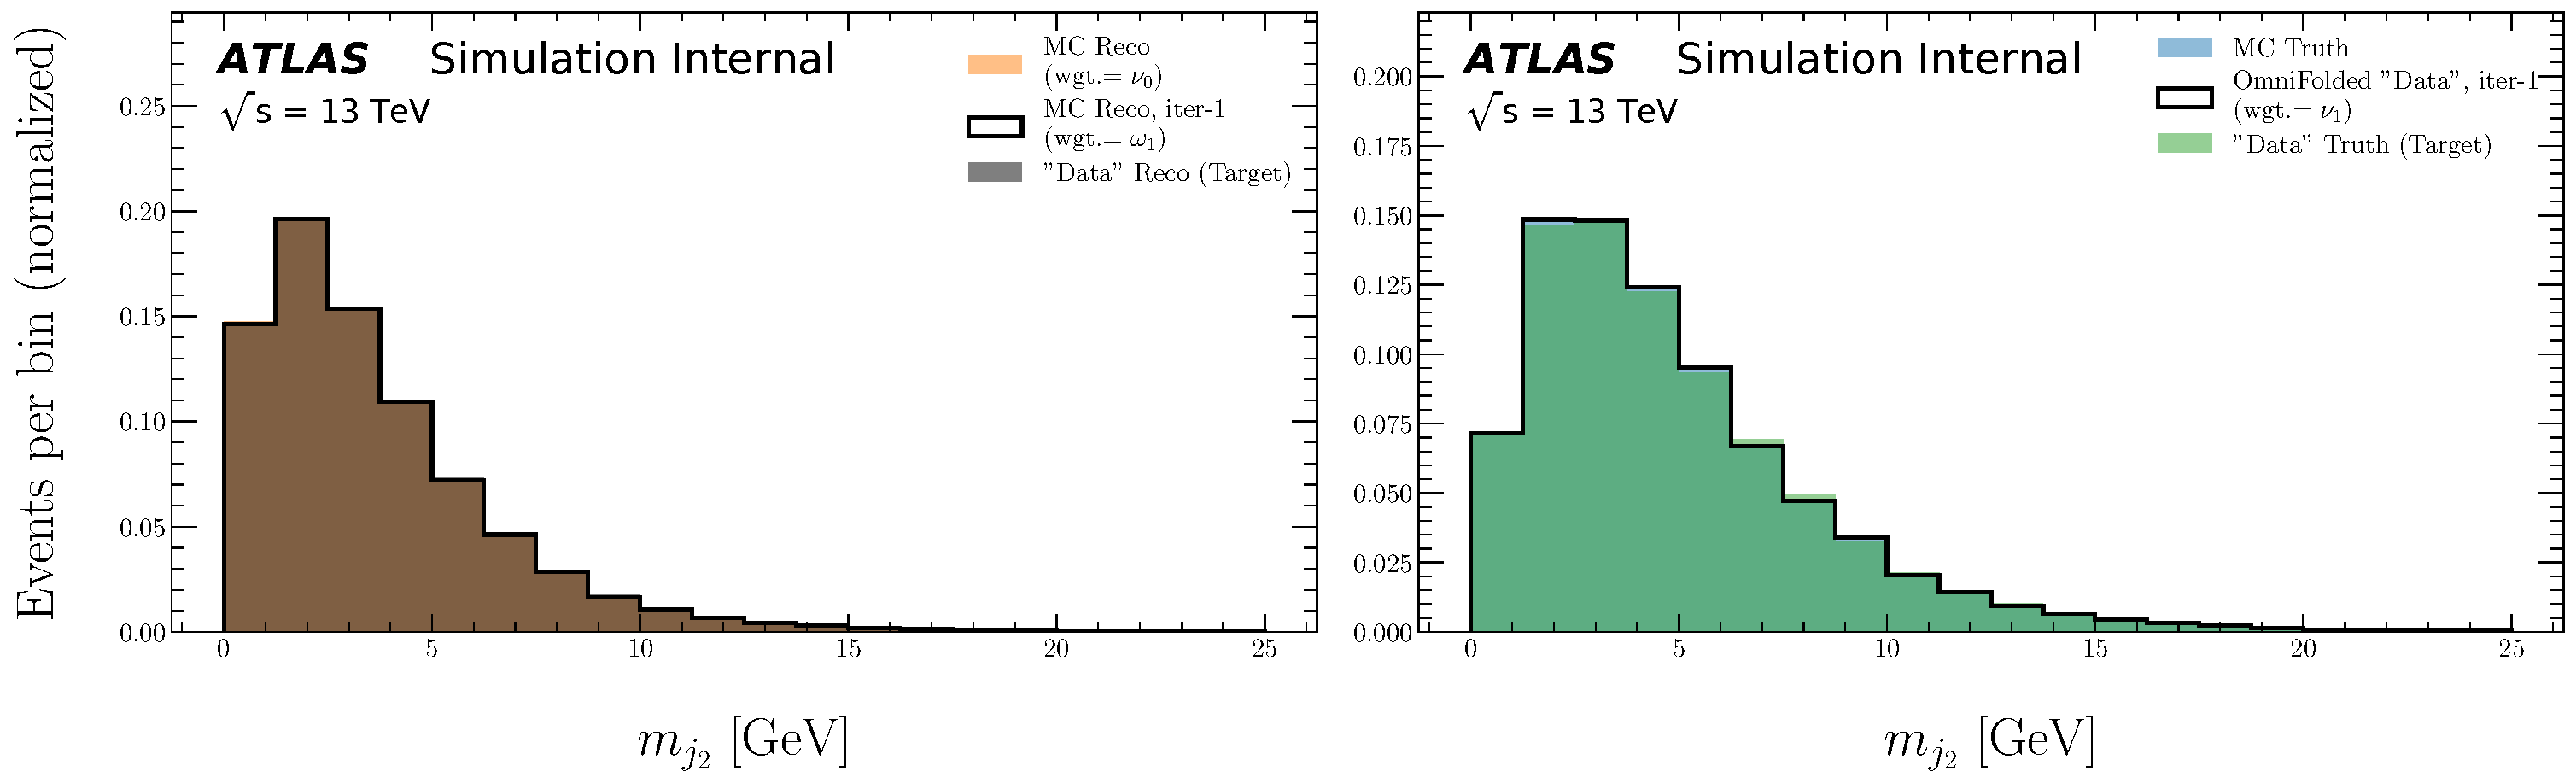
\includegraphics[width=0.95\textwidth]{figures/ATLASOmniFold-StressTest/ATLASOmniFold-TechnicalClosureTest/MultiFold/m_trackj2/ATLASOmniFold-TechnicalClosureTest-MultiFold-m_trackj2-Iteration01.pdf}}
\caption{A technical closure test for the mass of the subleading track jet using using MultiFold (16 observables are simultaneously unfolded).  The top plot show the input histograms and the bottom plots are the results after one iteration of OmniFold.  By construction the top left and top right histograms are statistically identical.}
\label{fig:technicalclosureMulti:mass2}
\end{figure}

\begin{figure}[h!]
\centering
\subfloat[Input histograms]{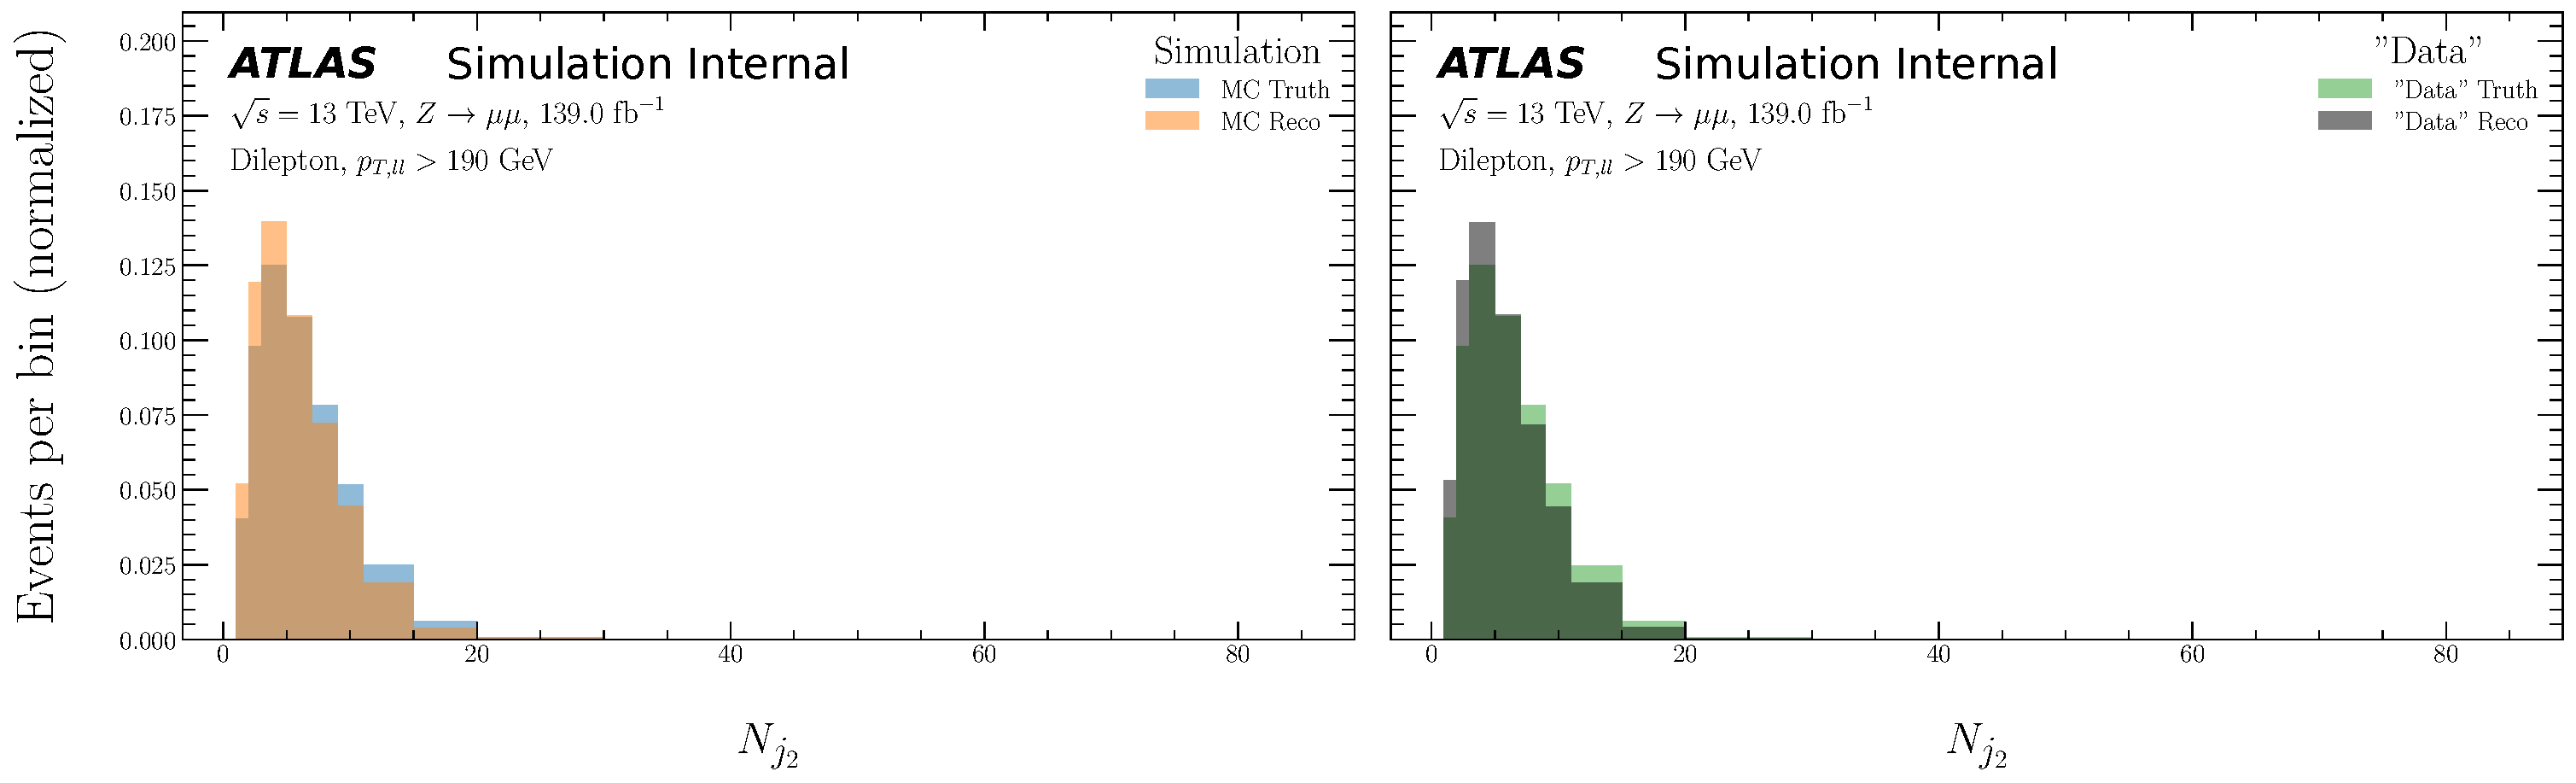
\includegraphics[width=0.95\textwidth]{figures/ATLASOmniFold-StressTest/ATLASOmniFold-TechnicalClosureTest/MultiFold/Ntracks_trackj2/ATLASOmniFold-TechnicalClosureTest-MultiFold-Ntracks_trackj2-Distributions.pdf}}\\
\subfloat[After 1 iteration]{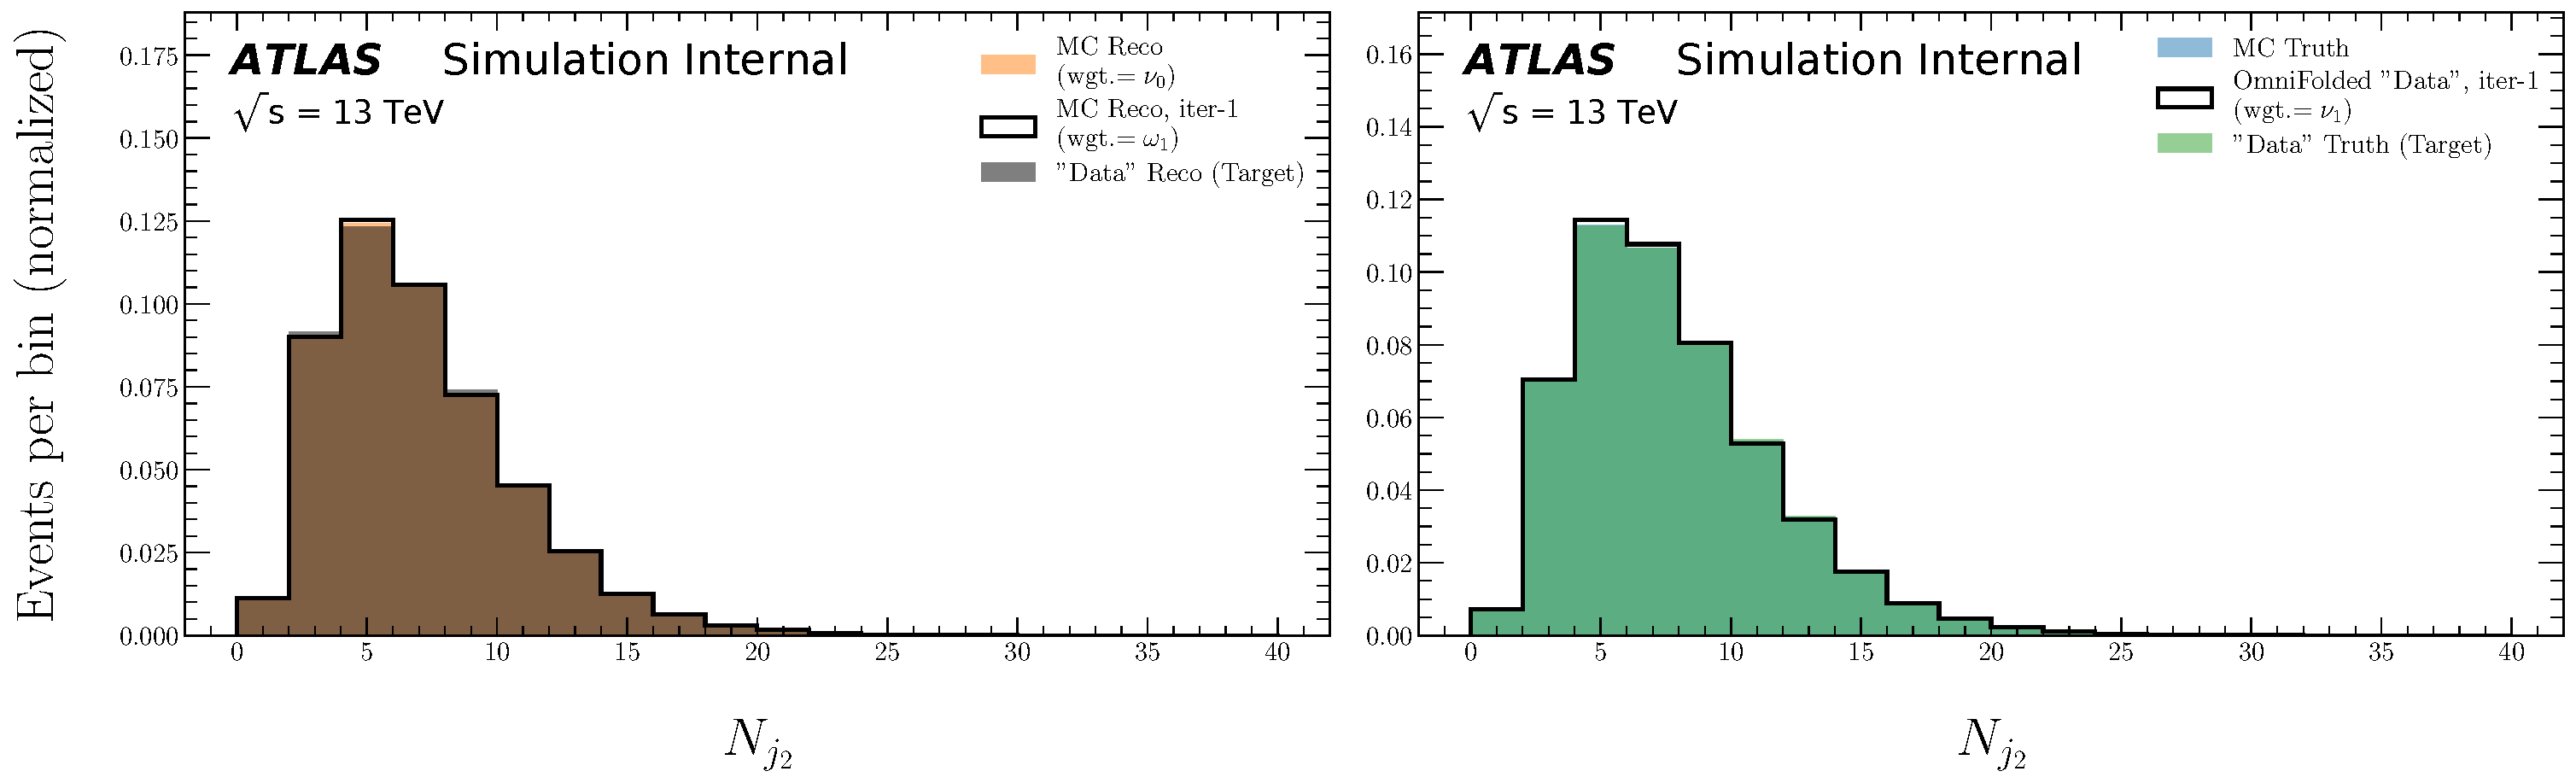
\includegraphics[width=0.95\textwidth]{figures/ATLASOmniFold-StressTest/ATLASOmniFold-TechnicalClosureTest/MultiFold/Ntracks_trackj2/ATLASOmniFold-TechnicalClosureTest-MultiFold-Ntracks_trackj2-Iteration01.pdf}}
\caption{A technical closure test for the number of tracks in the subleading track jet using MultiFold (16 observables are simultaneously unfolded).  The top plot show the input histograms and the bottom plots are the results after one iteration of OmniFold.  By construction the top left and top right histograms are statistically identical.}
\label{fig:technicalclosureMulti:ntracksjet2}
\end{figure}

\begin{figure}[h!]
\centering
\subfloat[Input histograms]{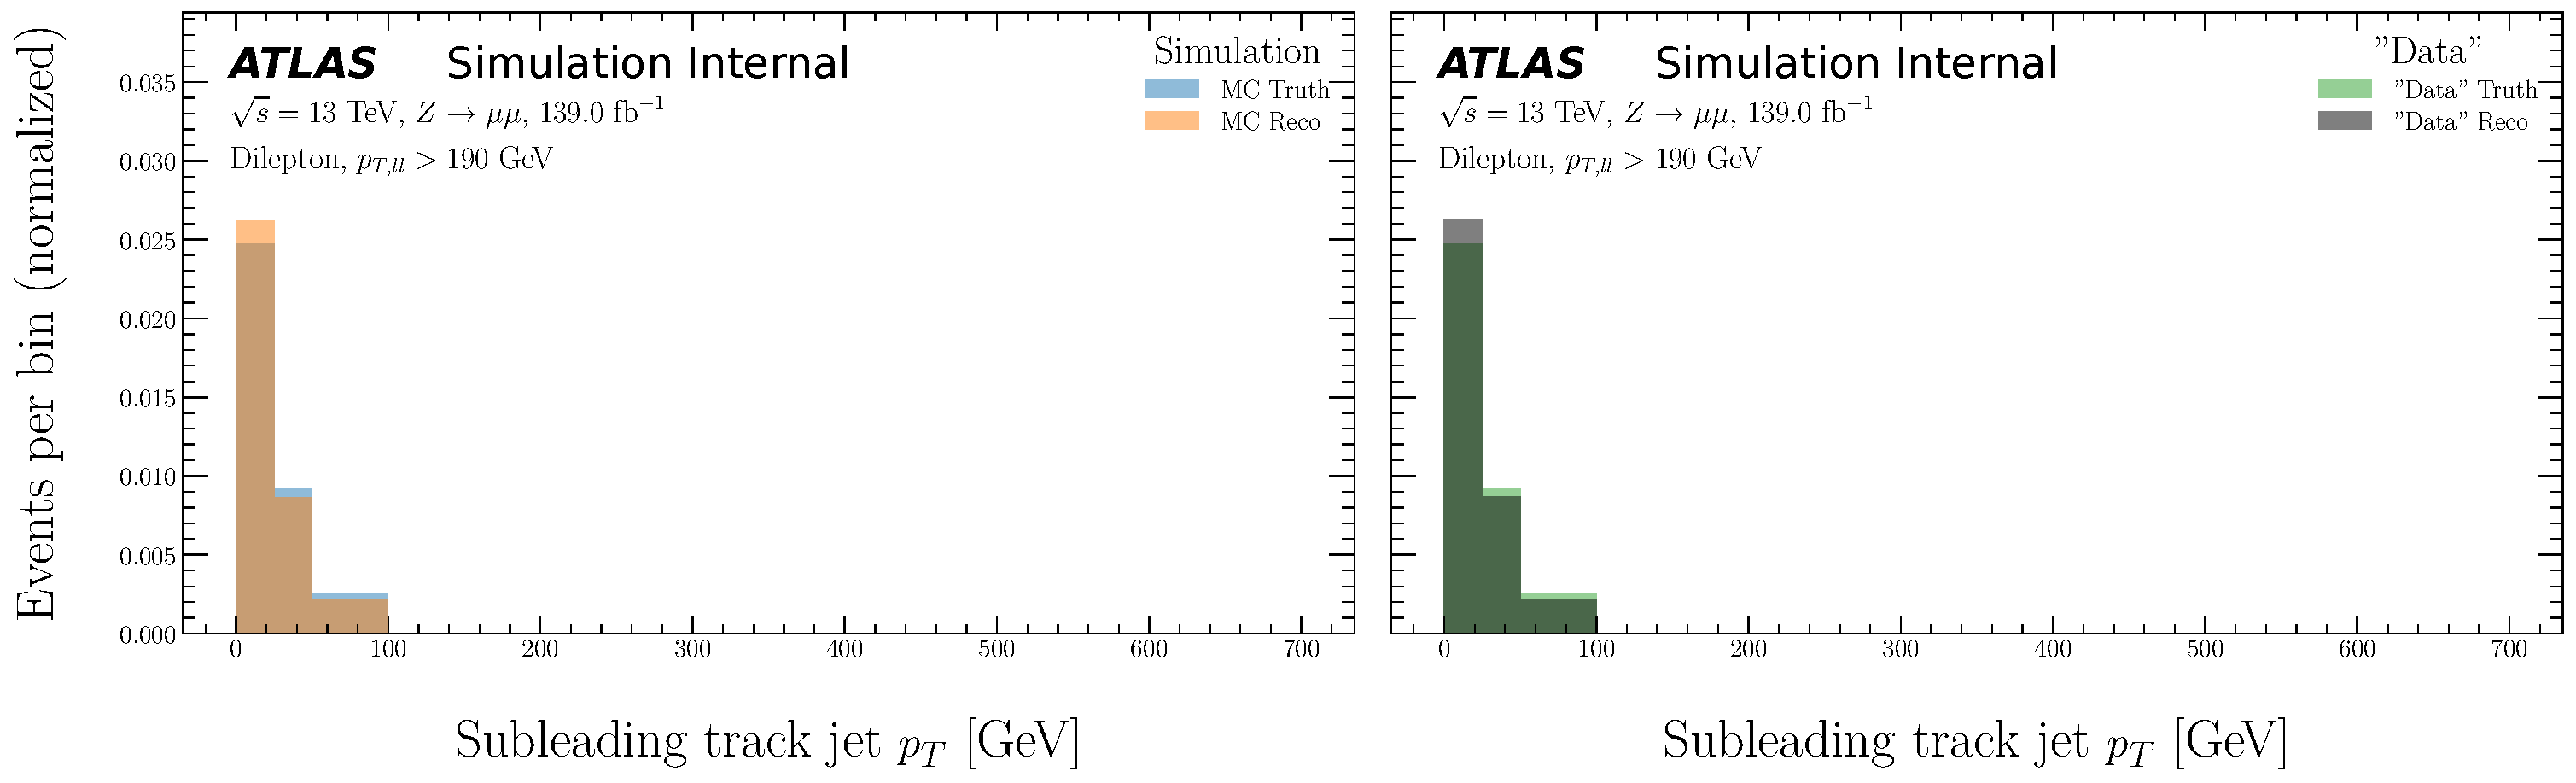
\includegraphics[width=0.95\textwidth]{figures/ATLASOmniFold-StressTest/ATLASOmniFold-TechnicalClosureTest/MultiFold/pT_trackj2/ATLASOmniFold-TechnicalClosureTest-MultiFold-pT_trackj2-Distributions.pdf}}\\
\subfloat[After 1 iteration]{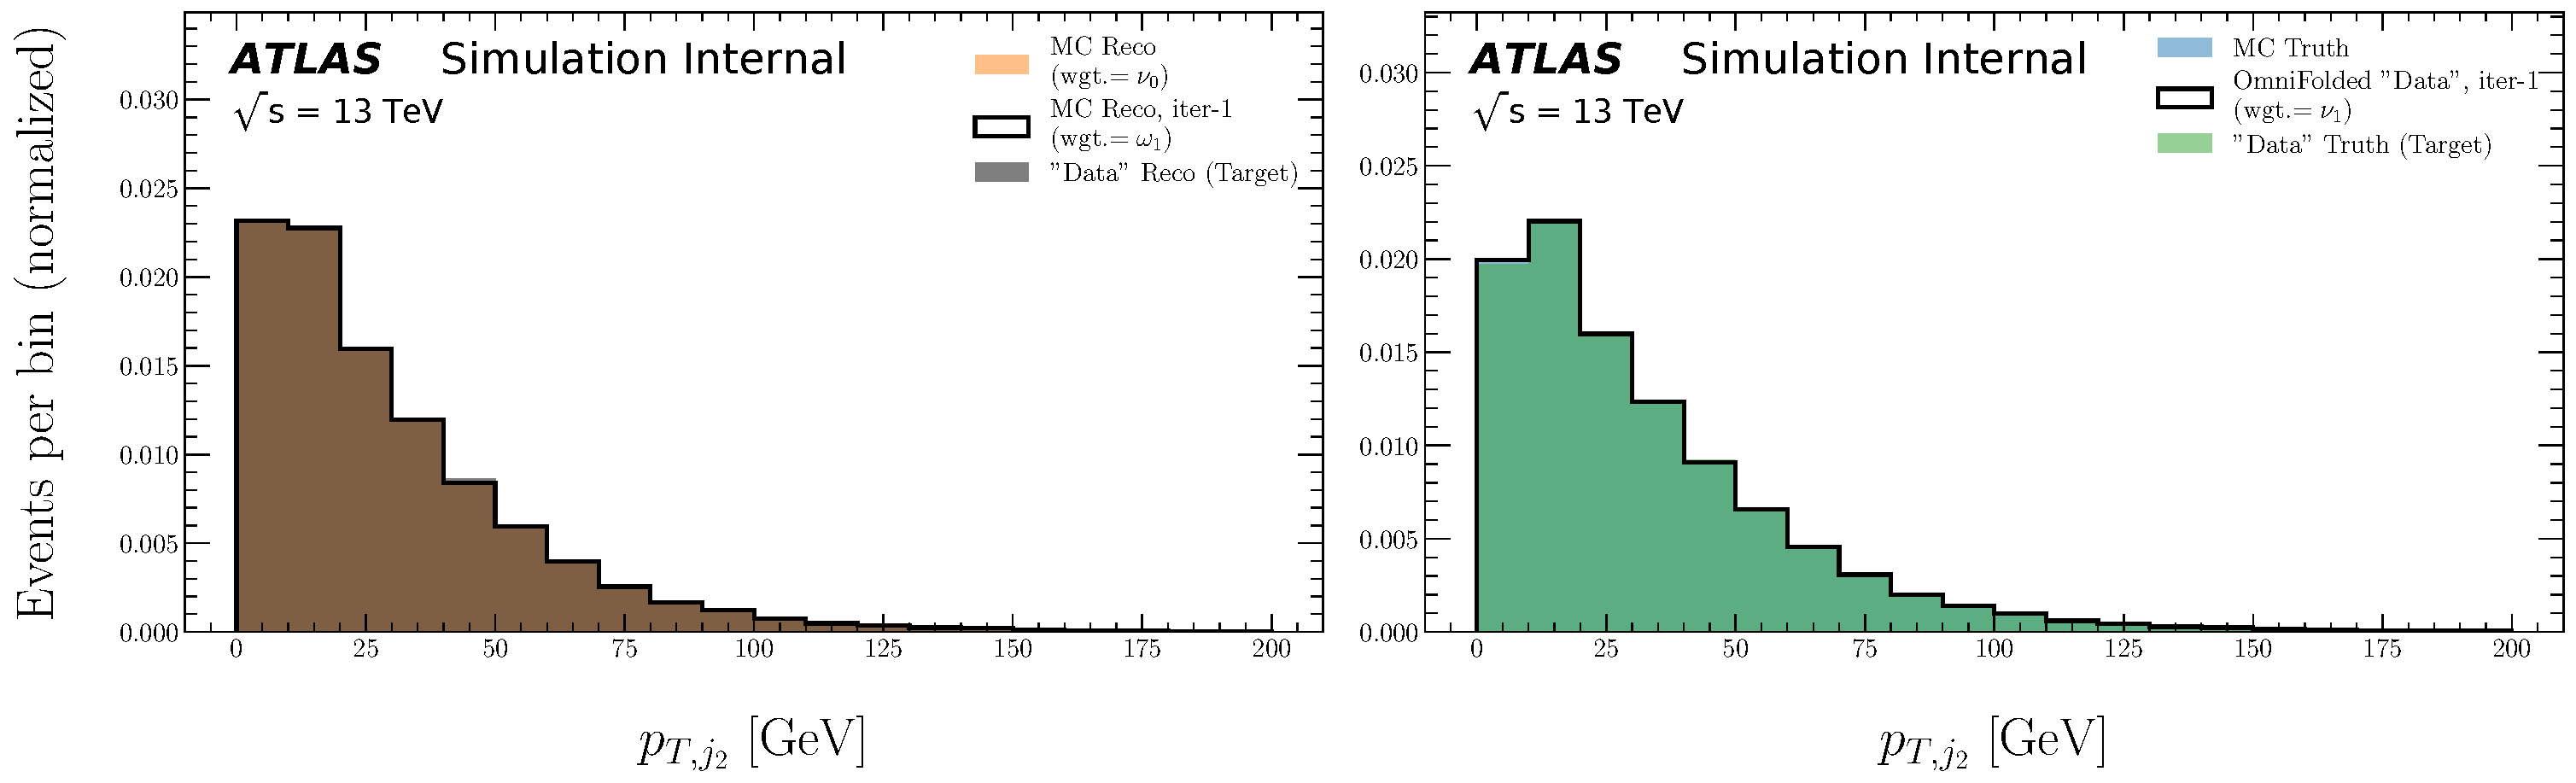
\includegraphics[width=0.95\textwidth]{figures/ATLASOmniFold-StressTest/ATLASOmniFold-TechnicalClosureTest/MultiFold/pT_trackj2/ATLASOmniFold-TechnicalClosureTest-MultiFold-pT_trackj2-Iteration01.pdf}}
\caption{A technical closure test for the $p_T$ of the subleading track jet using MultiFold (16 observables are simultaneously unfolded).  The top plot show the input histograms and the bottom plots are the results after one iteration of OmniFold.  By construction the top left and top right histograms are statistically identical.}
\label{fig:technicalclosureMulti:pT_trackj2}
\end{figure}

\begin{figure}[h!]
\centering
\subfloat[Input histograms]{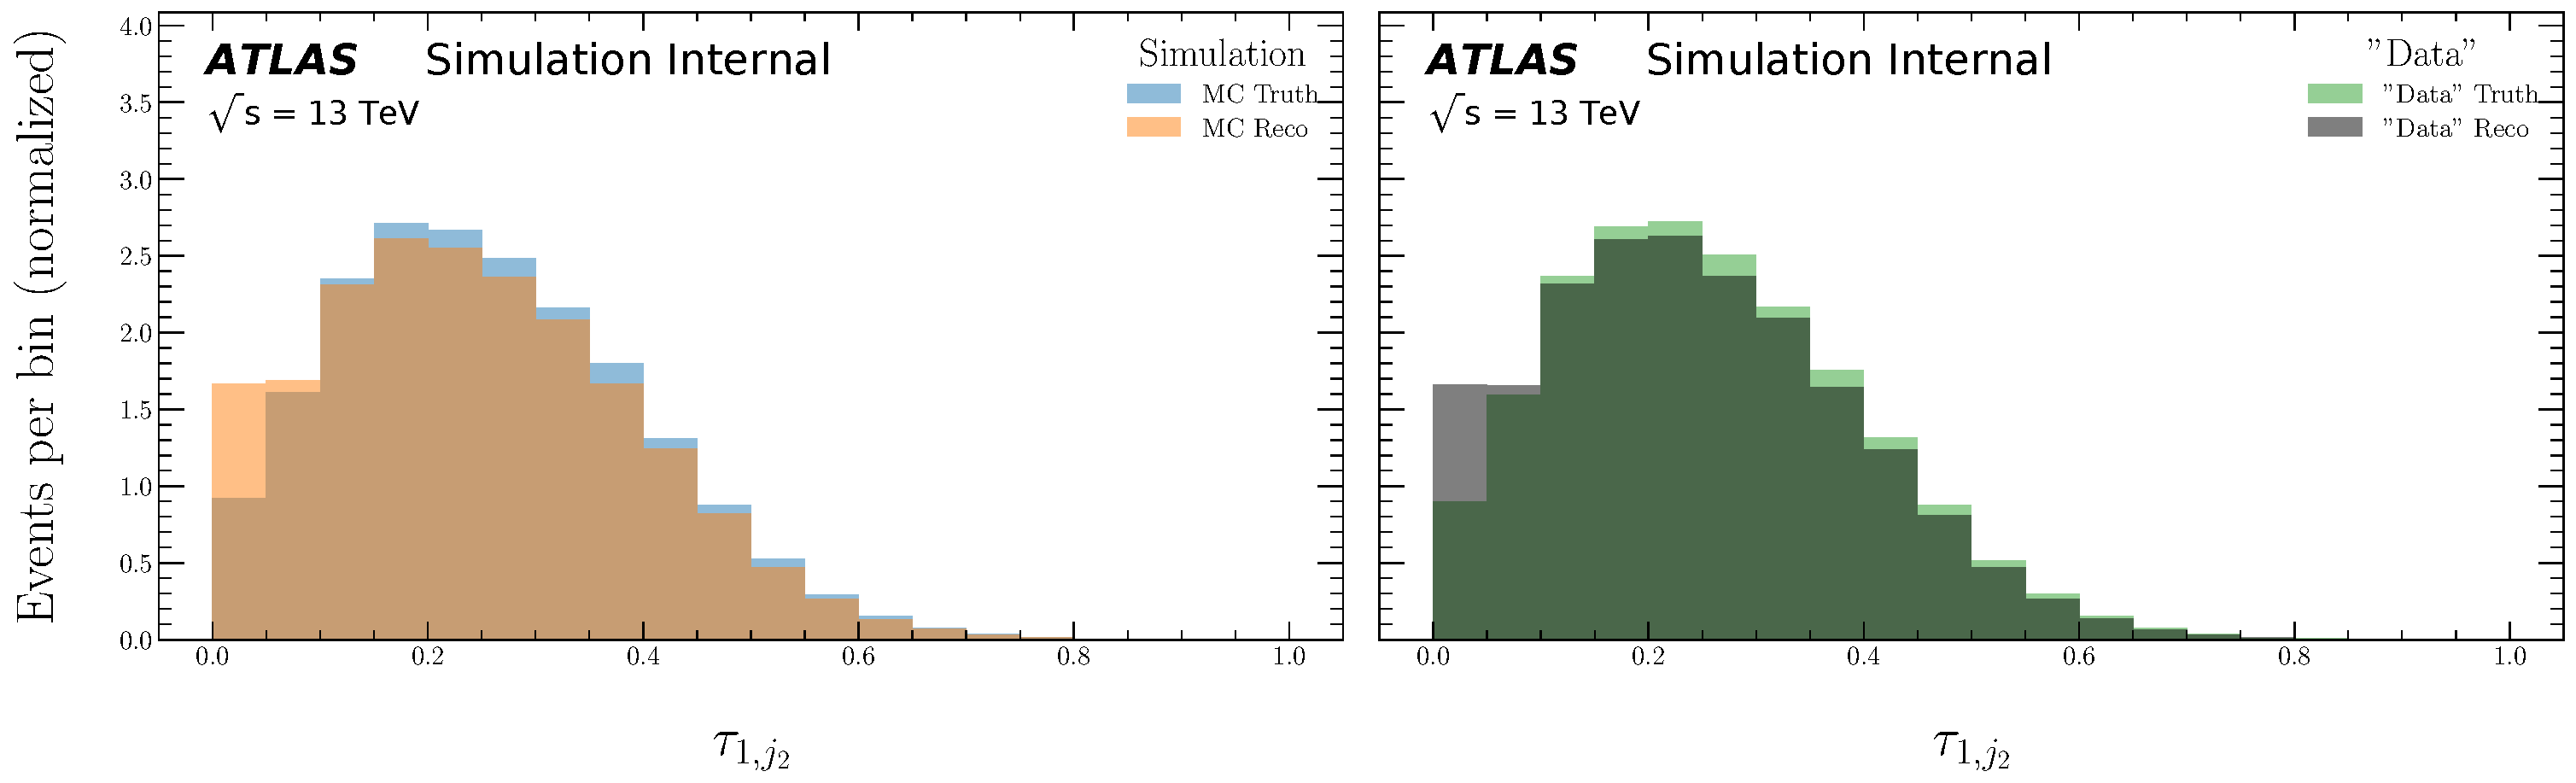
\includegraphics[width=0.89\textwidth]{figures/ATLASOmniFold-StressTest/ATLASOmniFold-TechnicalClosureTest/MultiFold/tau1_trackj2/ATLASOmniFold-TechnicalClosureTest-MultiFold-tau1_trackj2-Distributions.pdf}}\\
\subfloat[After 1 iteration]{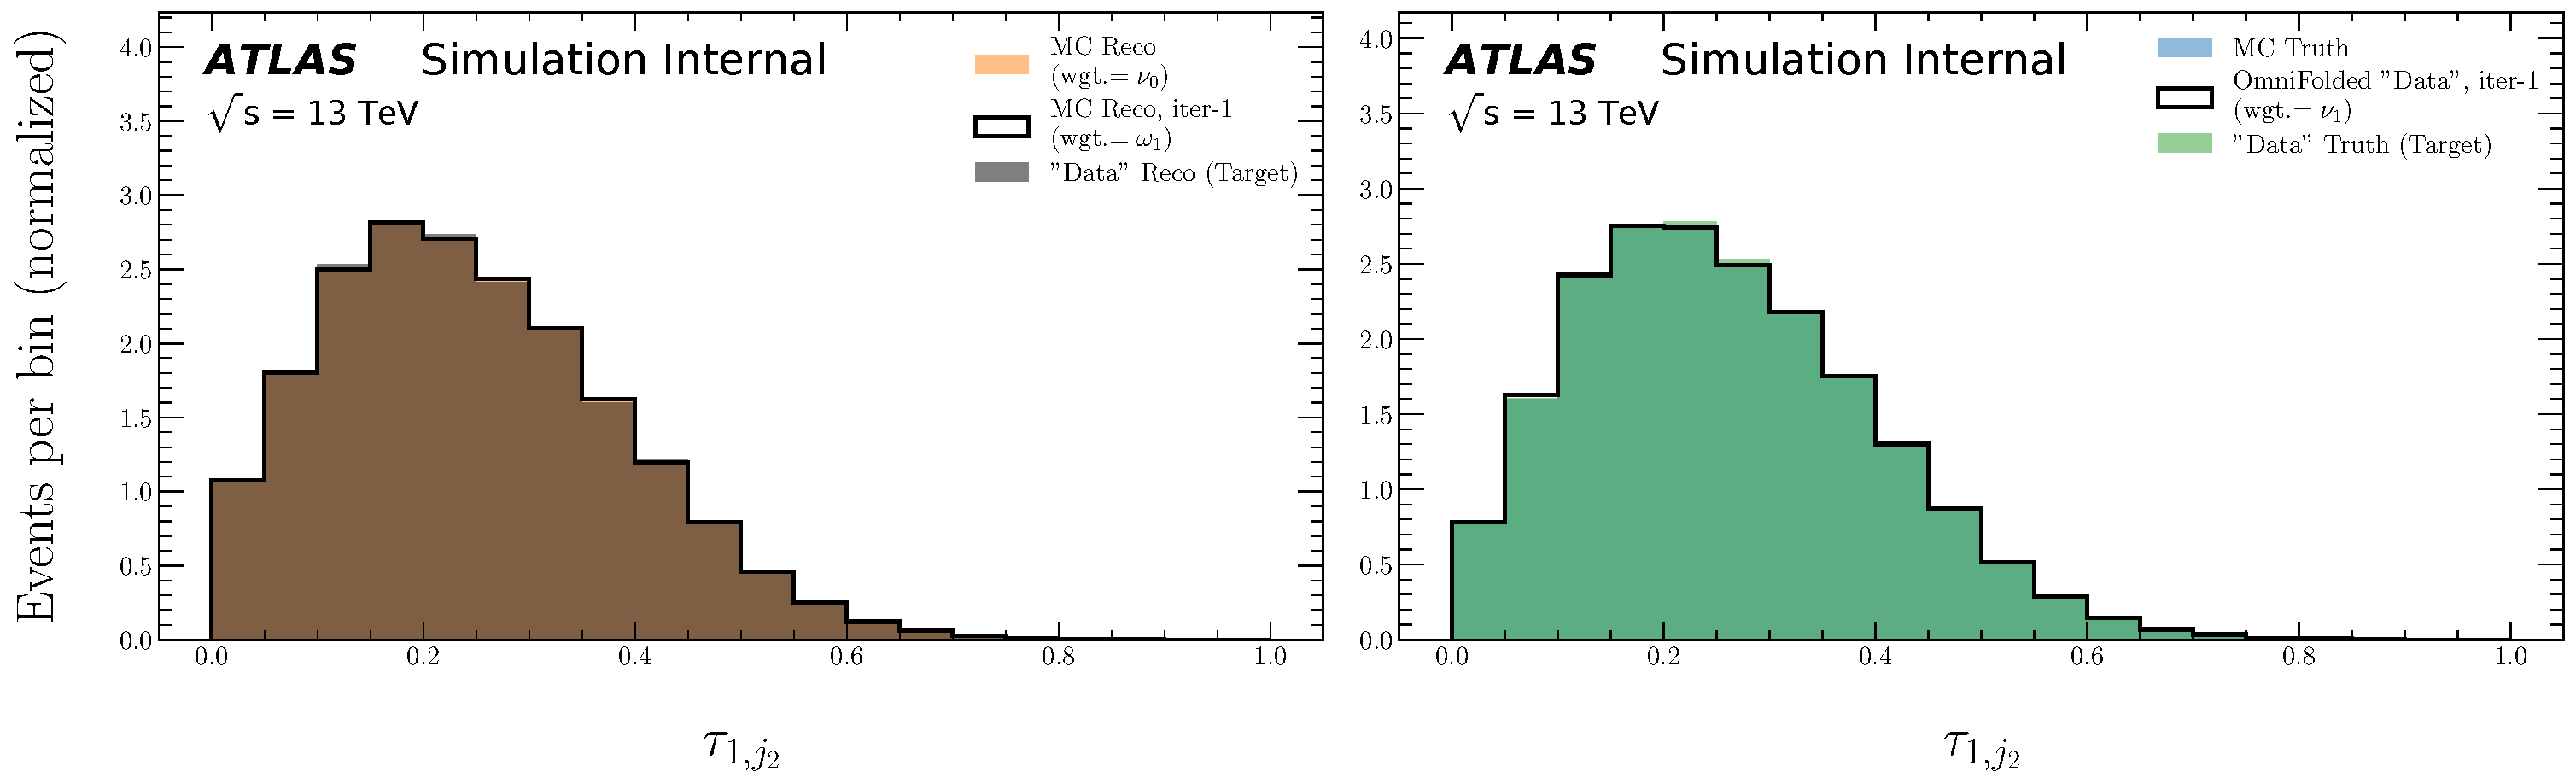
\includegraphics[width=0.95\textwidth]{figures/ATLASOmniFold-StressTest/ATLASOmniFold-TechnicalClosureTest/MultiFold/tau1_trackj2/ATLASOmniFold-TechnicalClosureTest-MultiFold-tau1_trackj2-Iteration01.pdf}}
\caption{A technical closure test for the $\tau_1$ of the subleading track jet using MultiFold (16 observables are simultaneously unfolded).  The top plot show the input histograms and the bottom plots are the results after one iteration of OmniFold.  By construction the top left and top right histograms are statistically identical.}
\label{fig:technicalclosureMulti:tau1_trackj2}
\end{figure}

\begin{figure}[h!]
\centering
\subfloat[Input histograms]{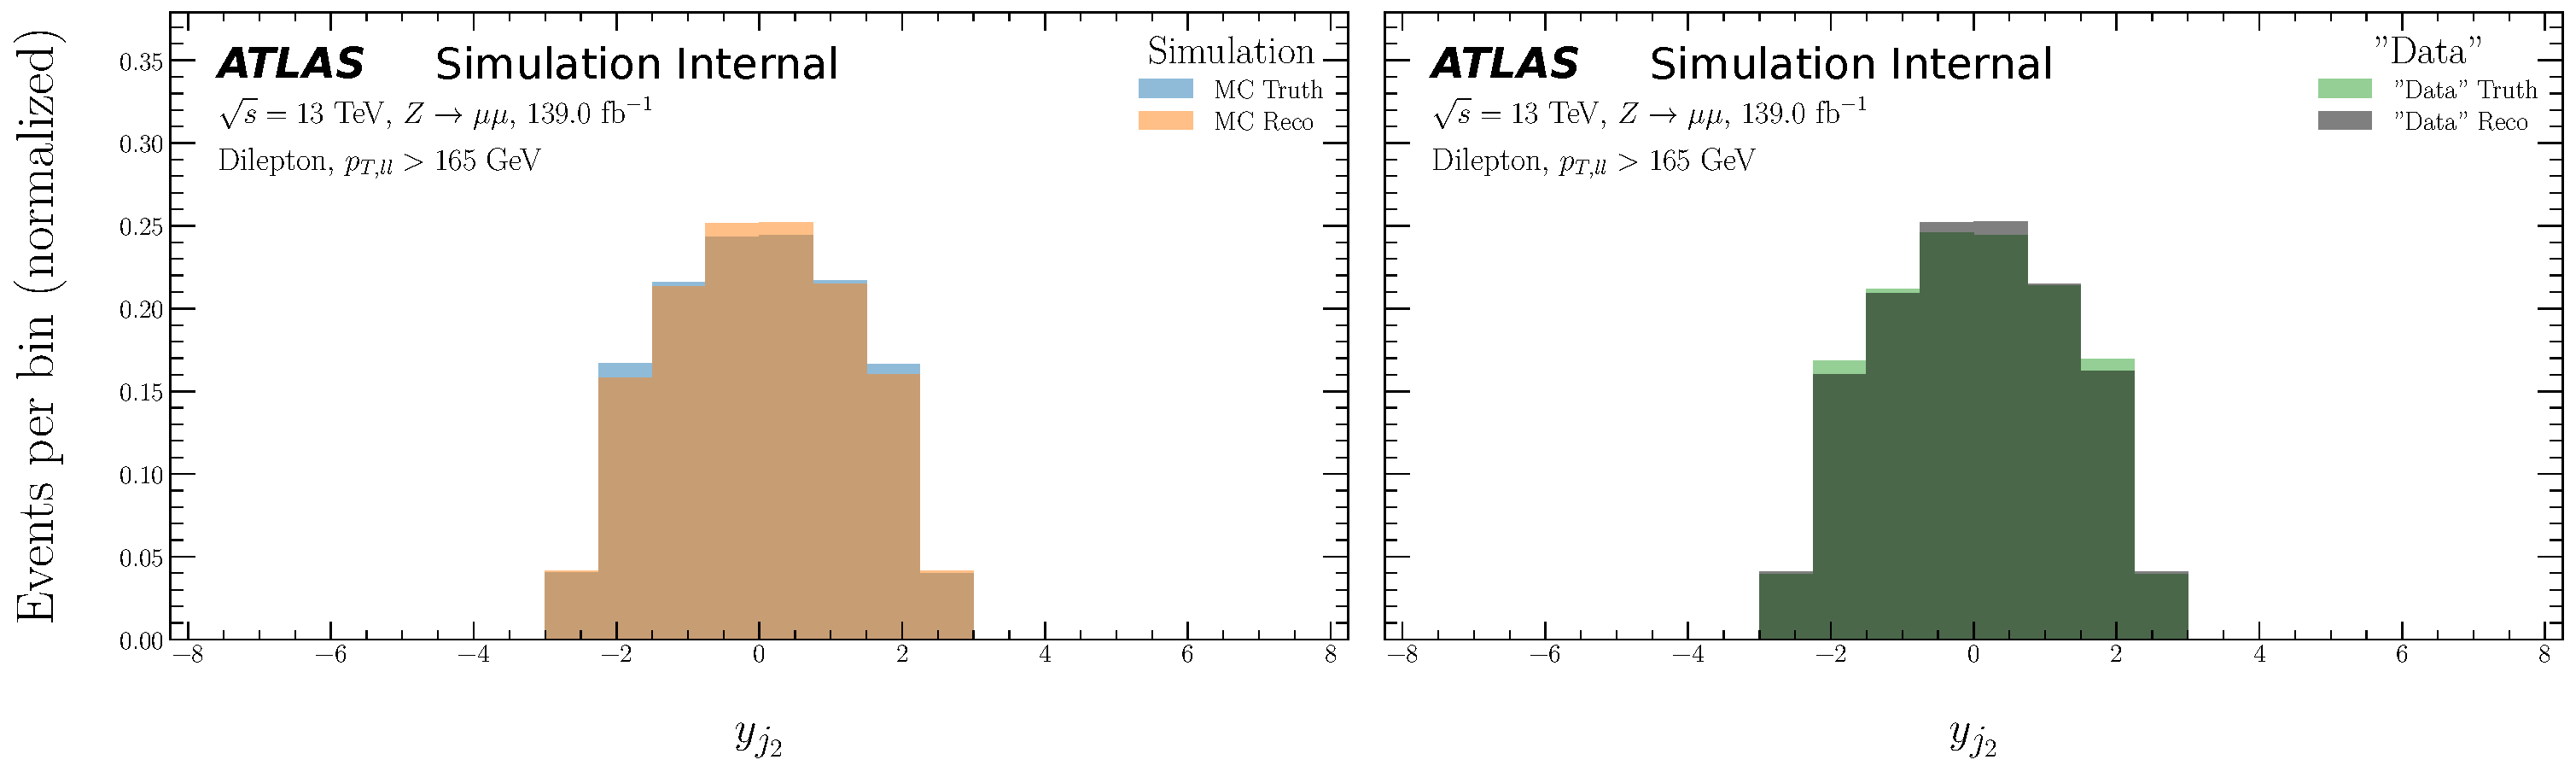
\includegraphics[width=0.95\textwidth]{figures/ATLASOmniFold-StressTest/ATLASOmniFold-TechnicalClosureTest/MultiFold/y_trackj2/ATLASOmniFold-TechnicalClosureTest-MultiFold-y_trackj2-Distributions.pdf}}\\
\subfloat[After 1 iteration]{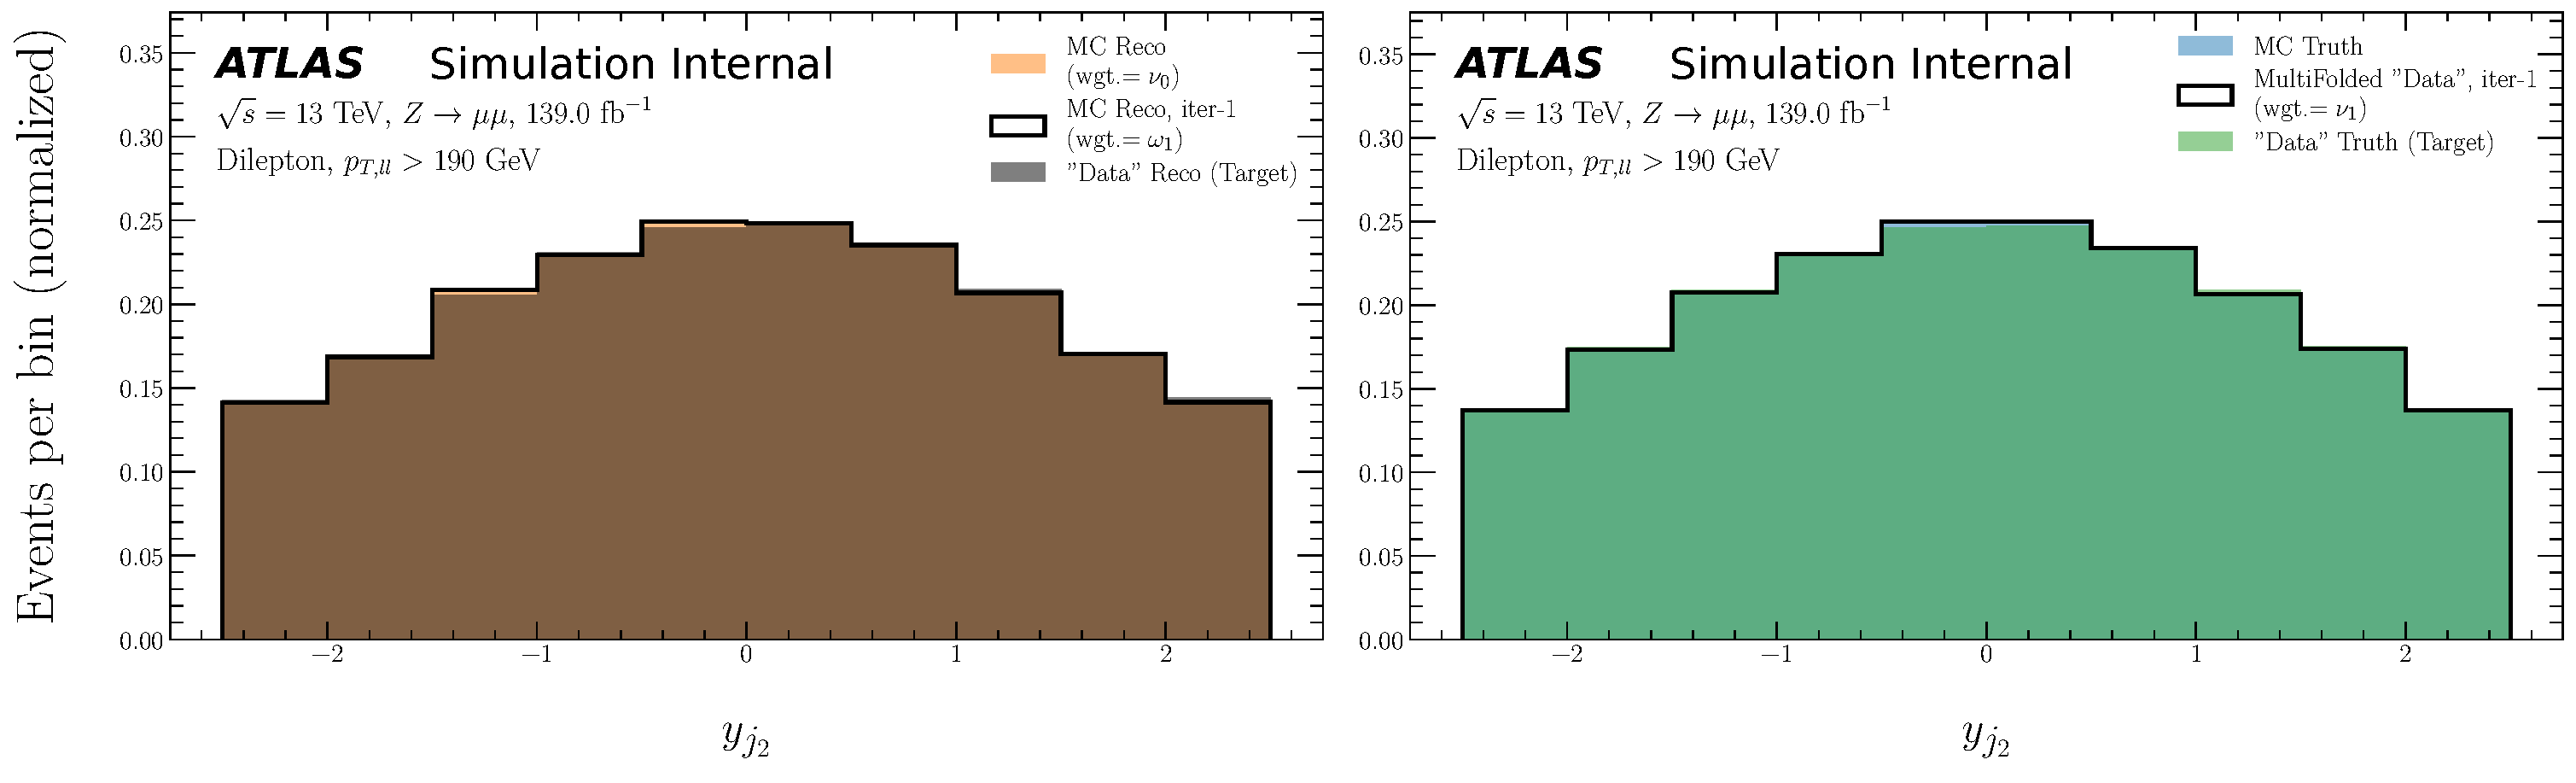
\includegraphics[width=0.95\textwidth]{figures/ATLASOmniFold-StressTest/ATLASOmniFold-TechnicalClosureTest/MultiFold/y_trackj2/ATLASOmniFold-TechnicalClosureTest-MultiFold-y_trackj2-Iteration01.pdf}}
\caption{A technical closure test for the rapidity of the subleading track jet using MultiFold (16 observables are simultaneously unfolded).  The top plot show the input histograms and the bottom plots are the results after one iteration of OmniFold.  By construction the top left and top right histograms are statistically identical.}
\label{fig:technicalclosureMulti:y_trackj2}
\end{figure}

\begin{figure}[h!]
\centering
\subfloat[Input histograms]{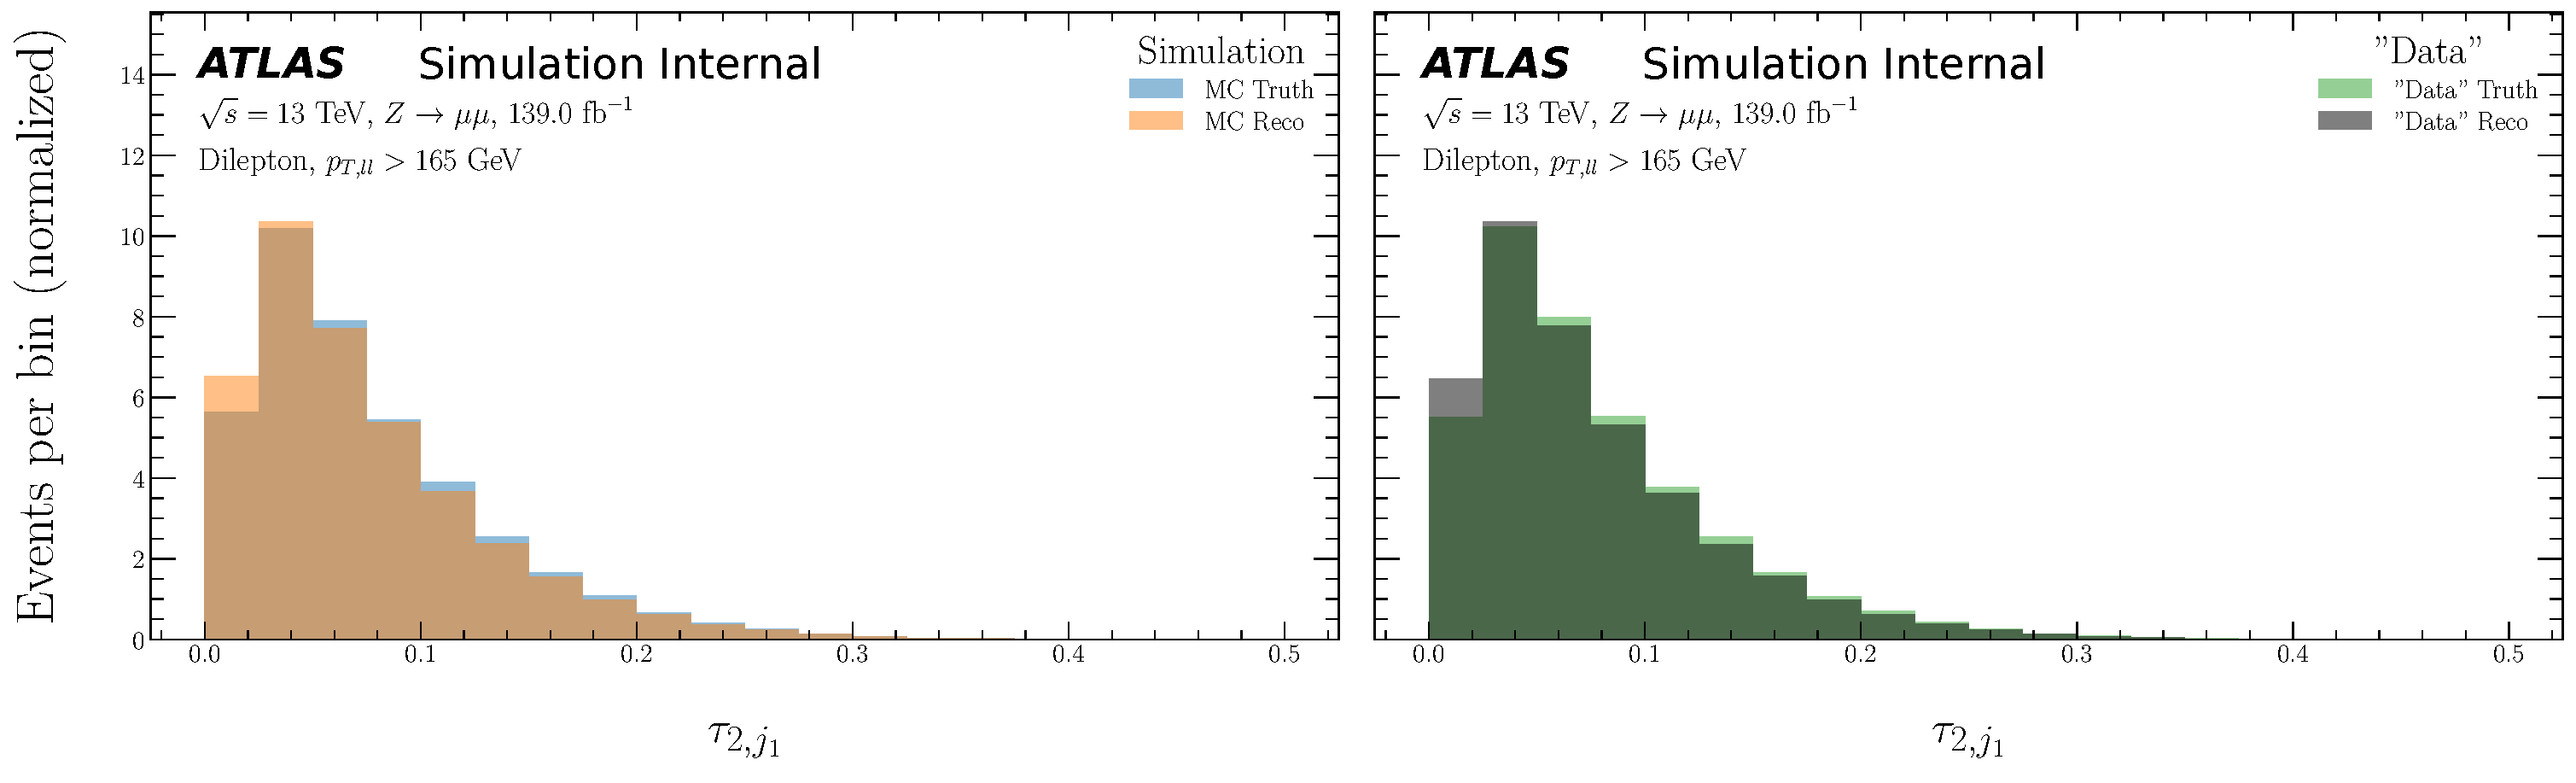
\includegraphics[width=0.89\textwidth]{figures/ATLASOmniFold-StressTest/ATLASOmniFold-TechnicalClosureTest/MultiFold/tau2_trackj1/ATLASOmniFold-TechnicalClosureTest-MultiFold-tau2_trackj1-Distributions.pdf}}\\
\subfloat[After 1 iteration]{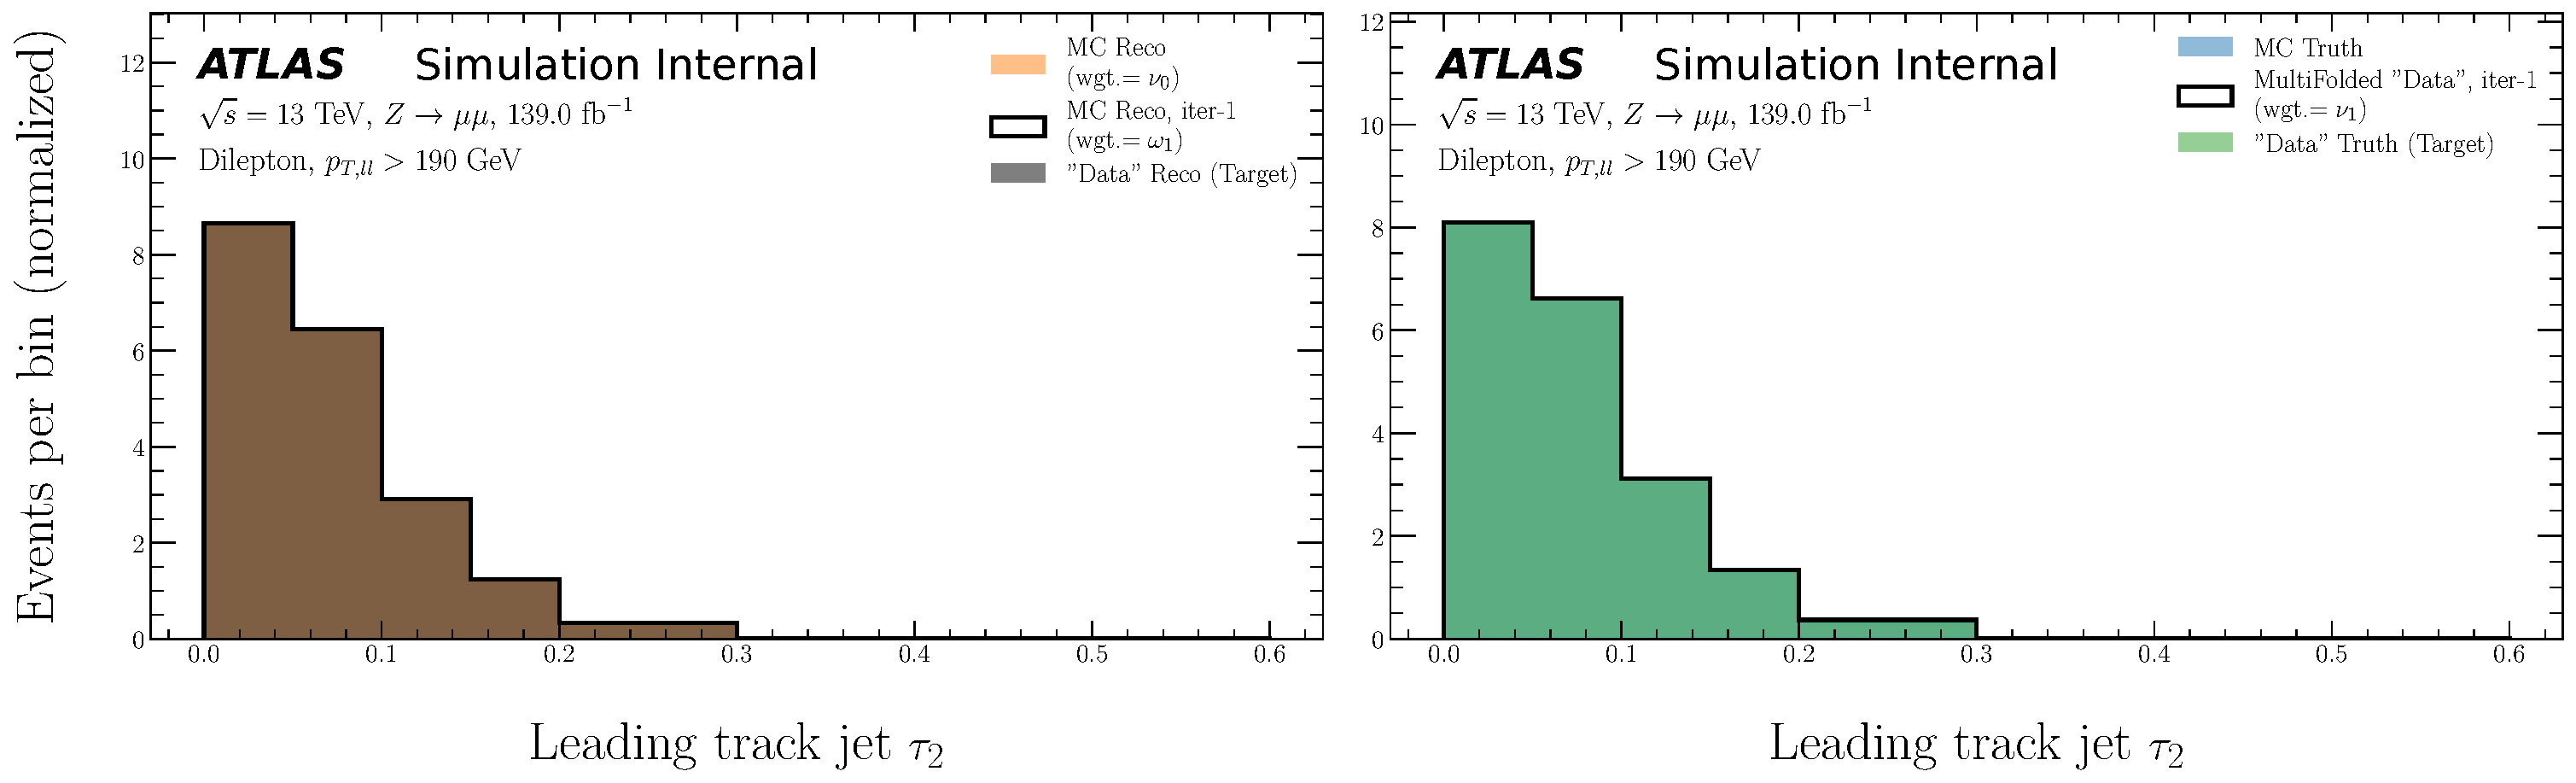
\includegraphics[width=0.95\textwidth]{figures/ATLASOmniFold-StressTest/ATLASOmniFold-TechnicalClosureTest/MultiFold/tau2_trackj1/ATLASOmniFold-TechnicalClosureTest-MultiFold-tau2_trackj1-Iteration01.pdf}}
\caption{A technical closure test for the $\tau_2$ of the leading track jet using MultiFold (16 observables are simultaneously unfolded).  The top plot show the input histograms and the bottom plots are the results after one iteration of OmniFold.  By construction the top left and top right histograms are statistically identical.}
\label{fig:technicalclosureMulti:tau2_trackj1}
\end{figure}

\begin{figure}[h!]
\centering
\subfloat[Input histograms]{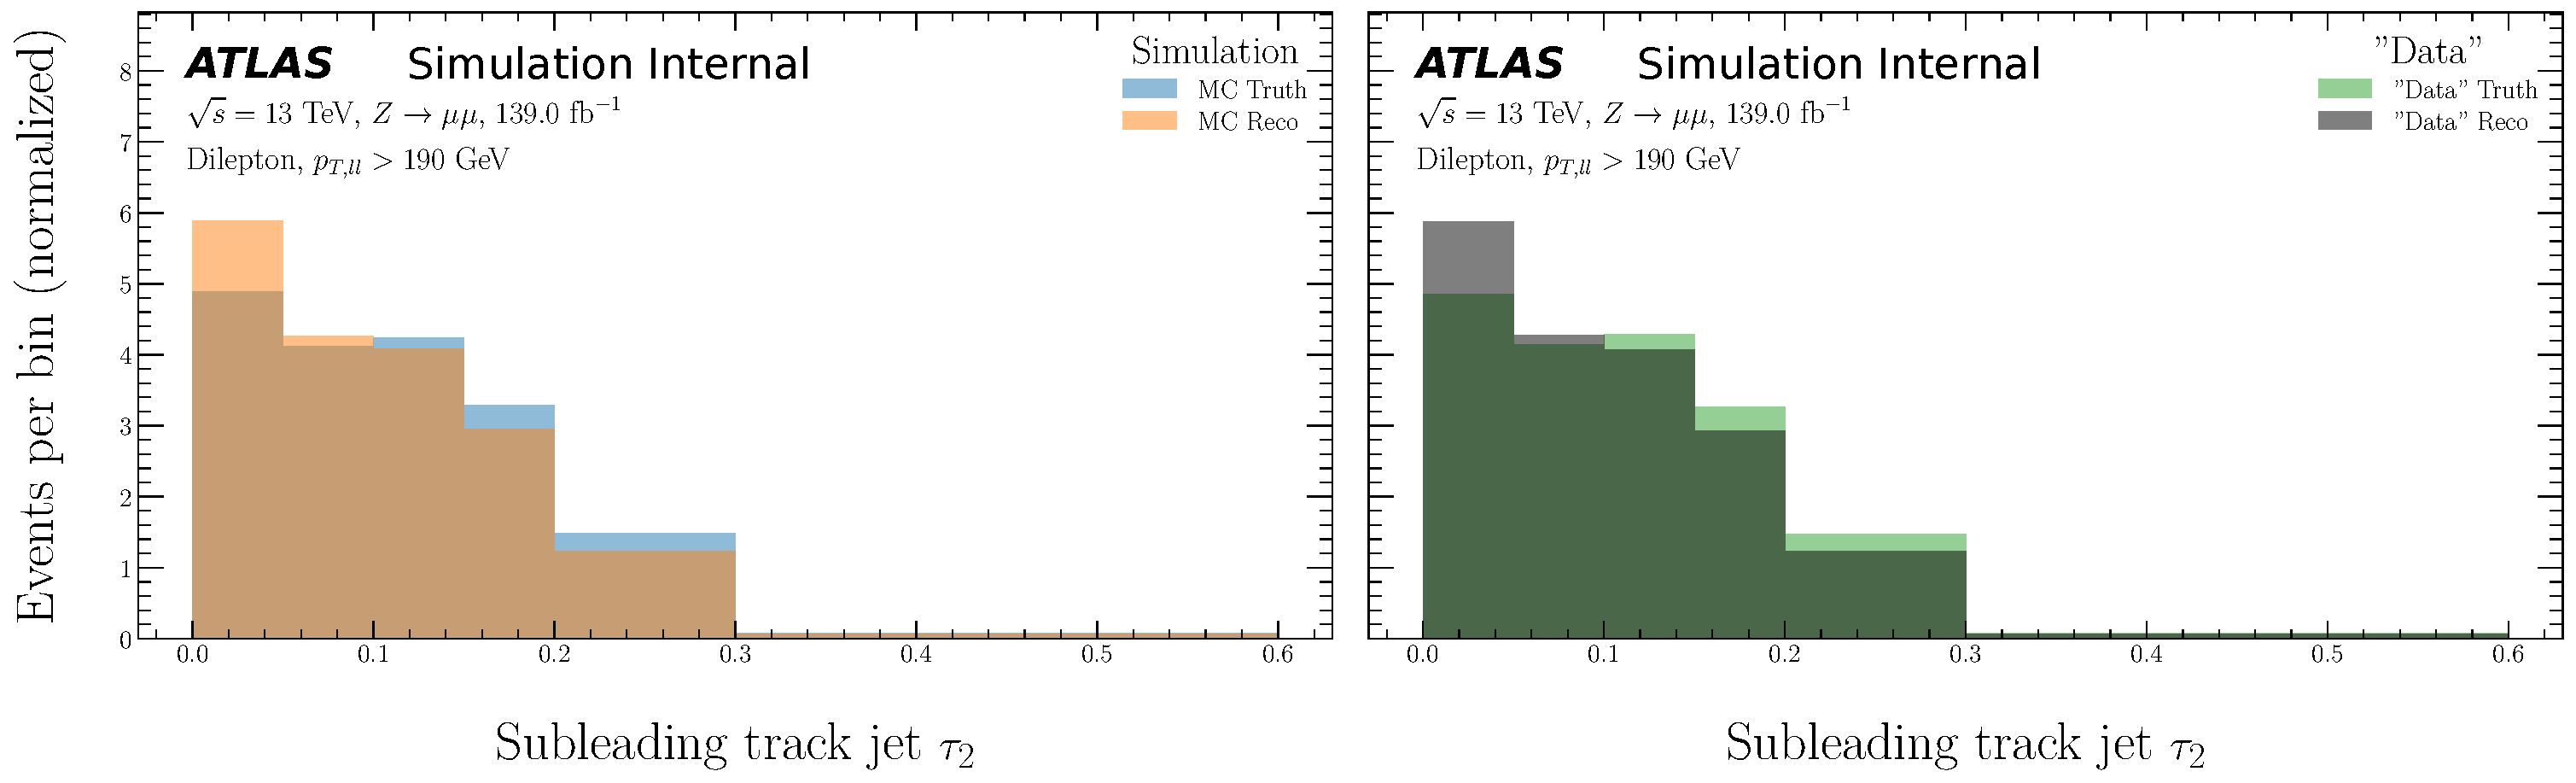
\includegraphics[width=0.89\textwidth]{figures/ATLASOmniFold-StressTest/ATLASOmniFold-TechnicalClosureTest/MultiFold/tau2_trackj2/ATLASOmniFold-TechnicalClosureTest-MultiFold-tau2_trackj2-Distributions.pdf}}\\
\subfloat[After 1 iteration]{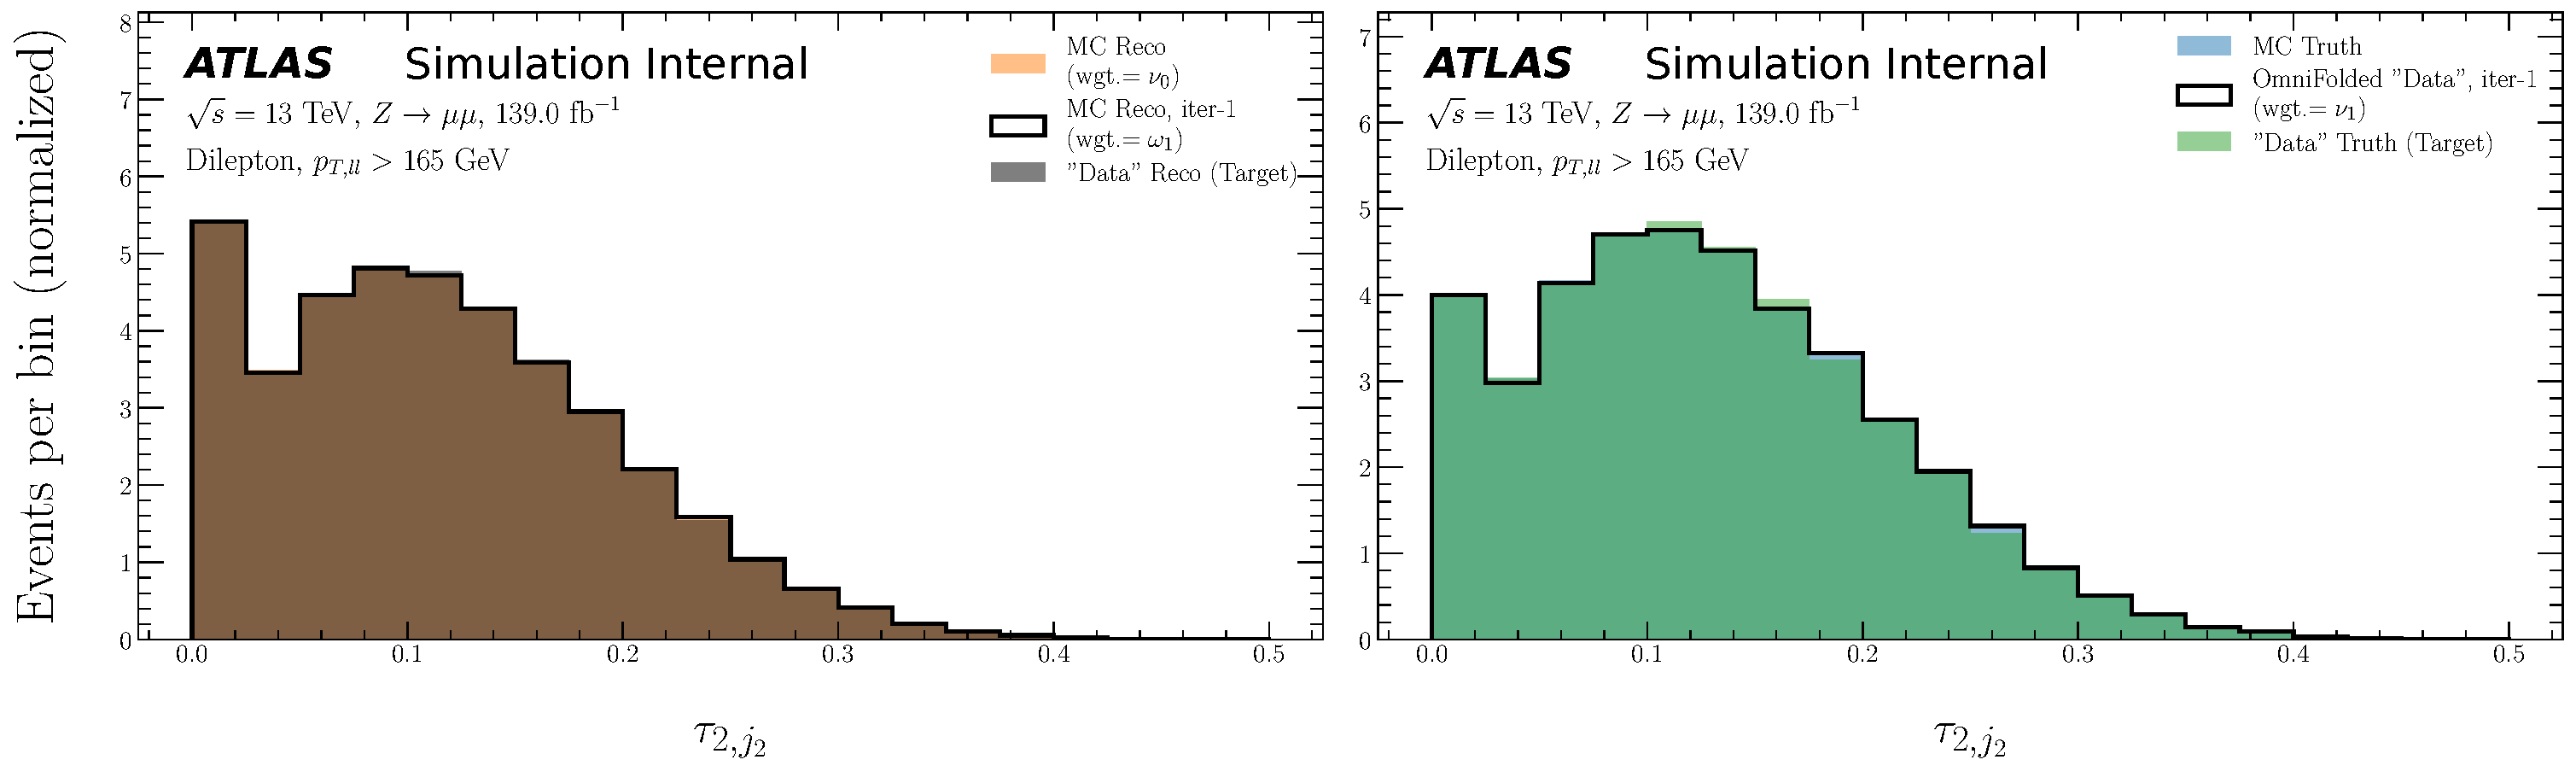
\includegraphics[width=0.95\textwidth]{figures/ATLASOmniFold-StressTest/ATLASOmniFold-TechnicalClosureTest/MultiFold/tau2_trackj2/ATLASOmniFold-TechnicalClosureTest-MultiFold-tau2_trackj2-Iteration01.pdf}}
\caption{A technical closure test for the $\tau_2$ of the subleading track jet using MultiFold (16 observables are simultaneously unfolded).  The top plot show the input histograms and the bottom plots are the results after one iteration of OmniFold.  By construction the top left and top right histograms are statistically identical.}
\label{fig:technicalclosureMulti:tau2_trackj2}
\end{figure}

\begin{figure}[h!]
\centering
\subfloat[Input histograms]{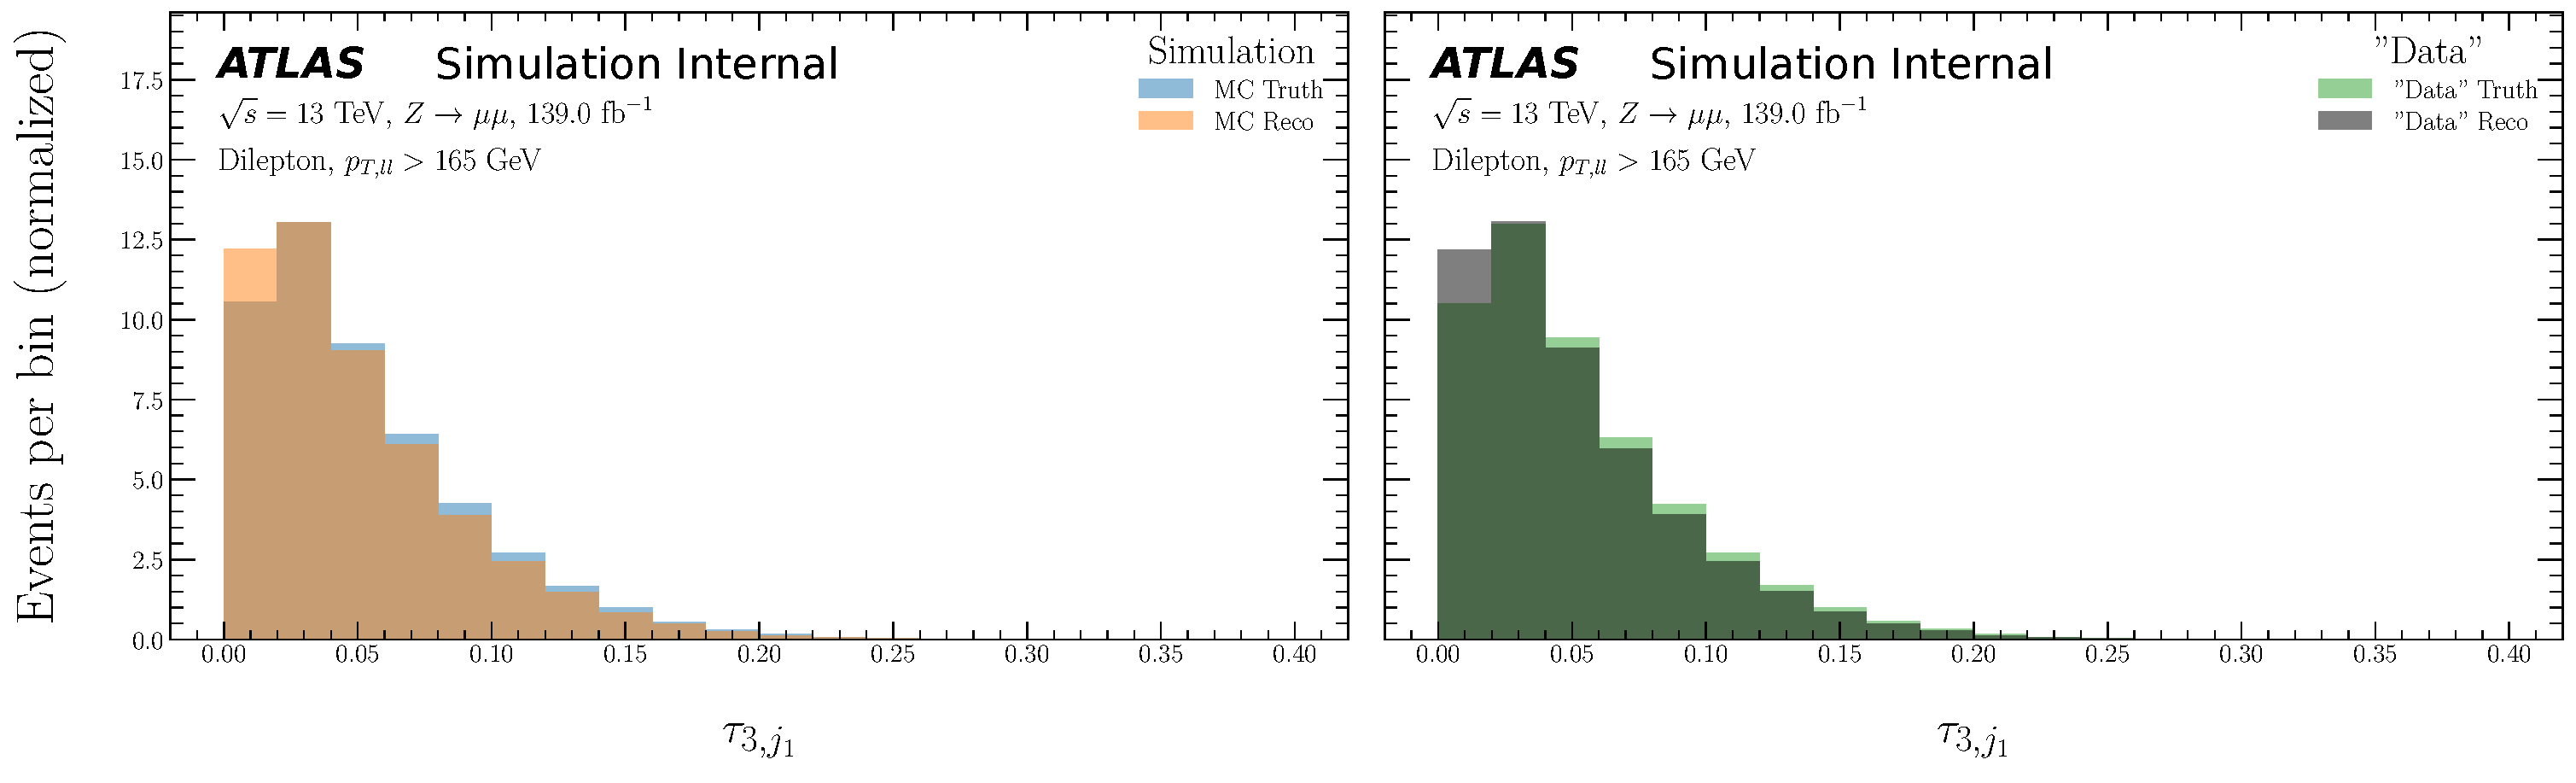
\includegraphics[width=0.89\textwidth]{figures/ATLASOmniFold-StressTest/ATLASOmniFold-TechnicalClosureTest/MultiFold/tau3_trackj1/ATLASOmniFold-TechnicalClosureTest-MultiFold-tau3_trackj1-Distributions.pdf}}\\
\subfloat[After 1 iteration]{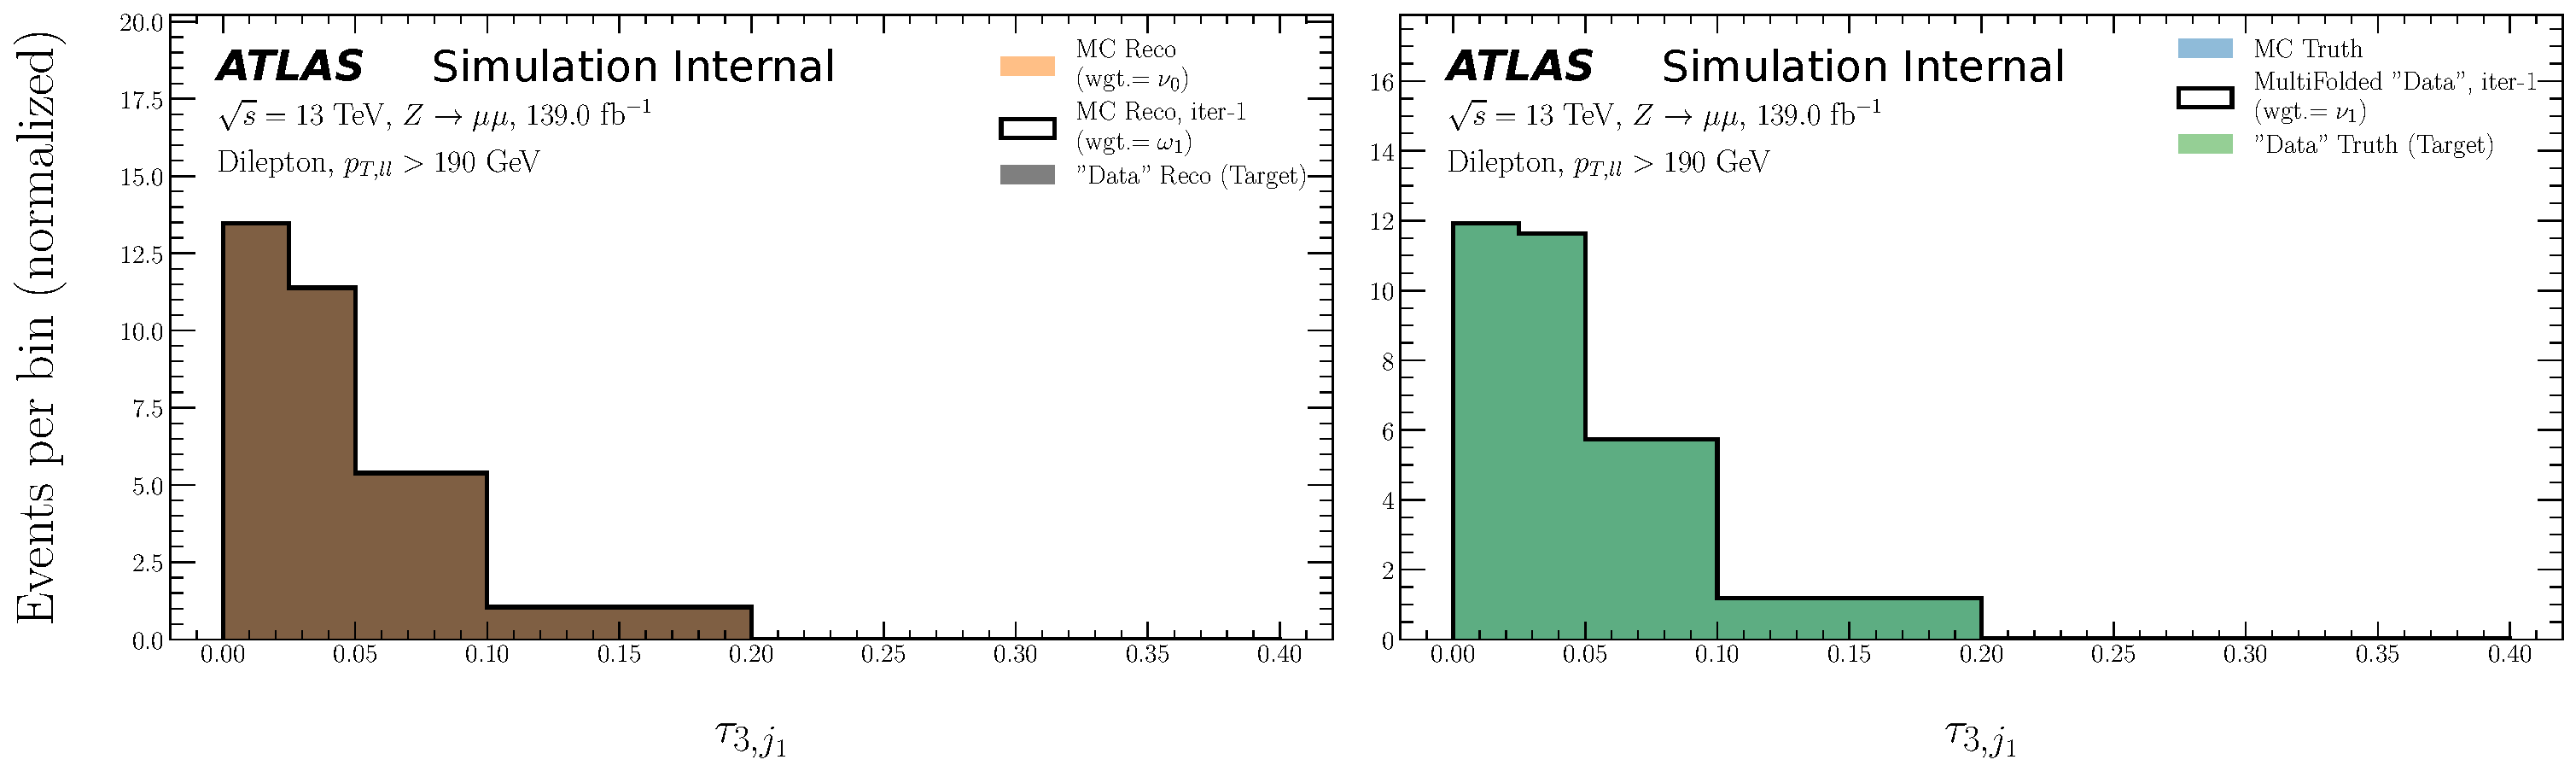
\includegraphics[width=0.95\textwidth]{figures/ATLASOmniFold-StressTest/ATLASOmniFold-TechnicalClosureTest/MultiFold/tau3_trackj1/ATLASOmniFold-TechnicalClosureTest-MultiFold-tau3_trackj1-Iteration01.pdf}}
\caption{A technical closure test for the $\tau_3$ of the leading track jet using MultiFold (16 observables are simultaneously unfolded).  The top plot show the input histograms and the bottom plots are the results after one iteration of OmniFold.  By construction the top left and top right histograms are statistically identical.}
\label{fig:technicalclosureMulti:tau3_trackj1}
\end{figure}

\begin{figure}[h!]
\centering
\subfloat[Input histograms]{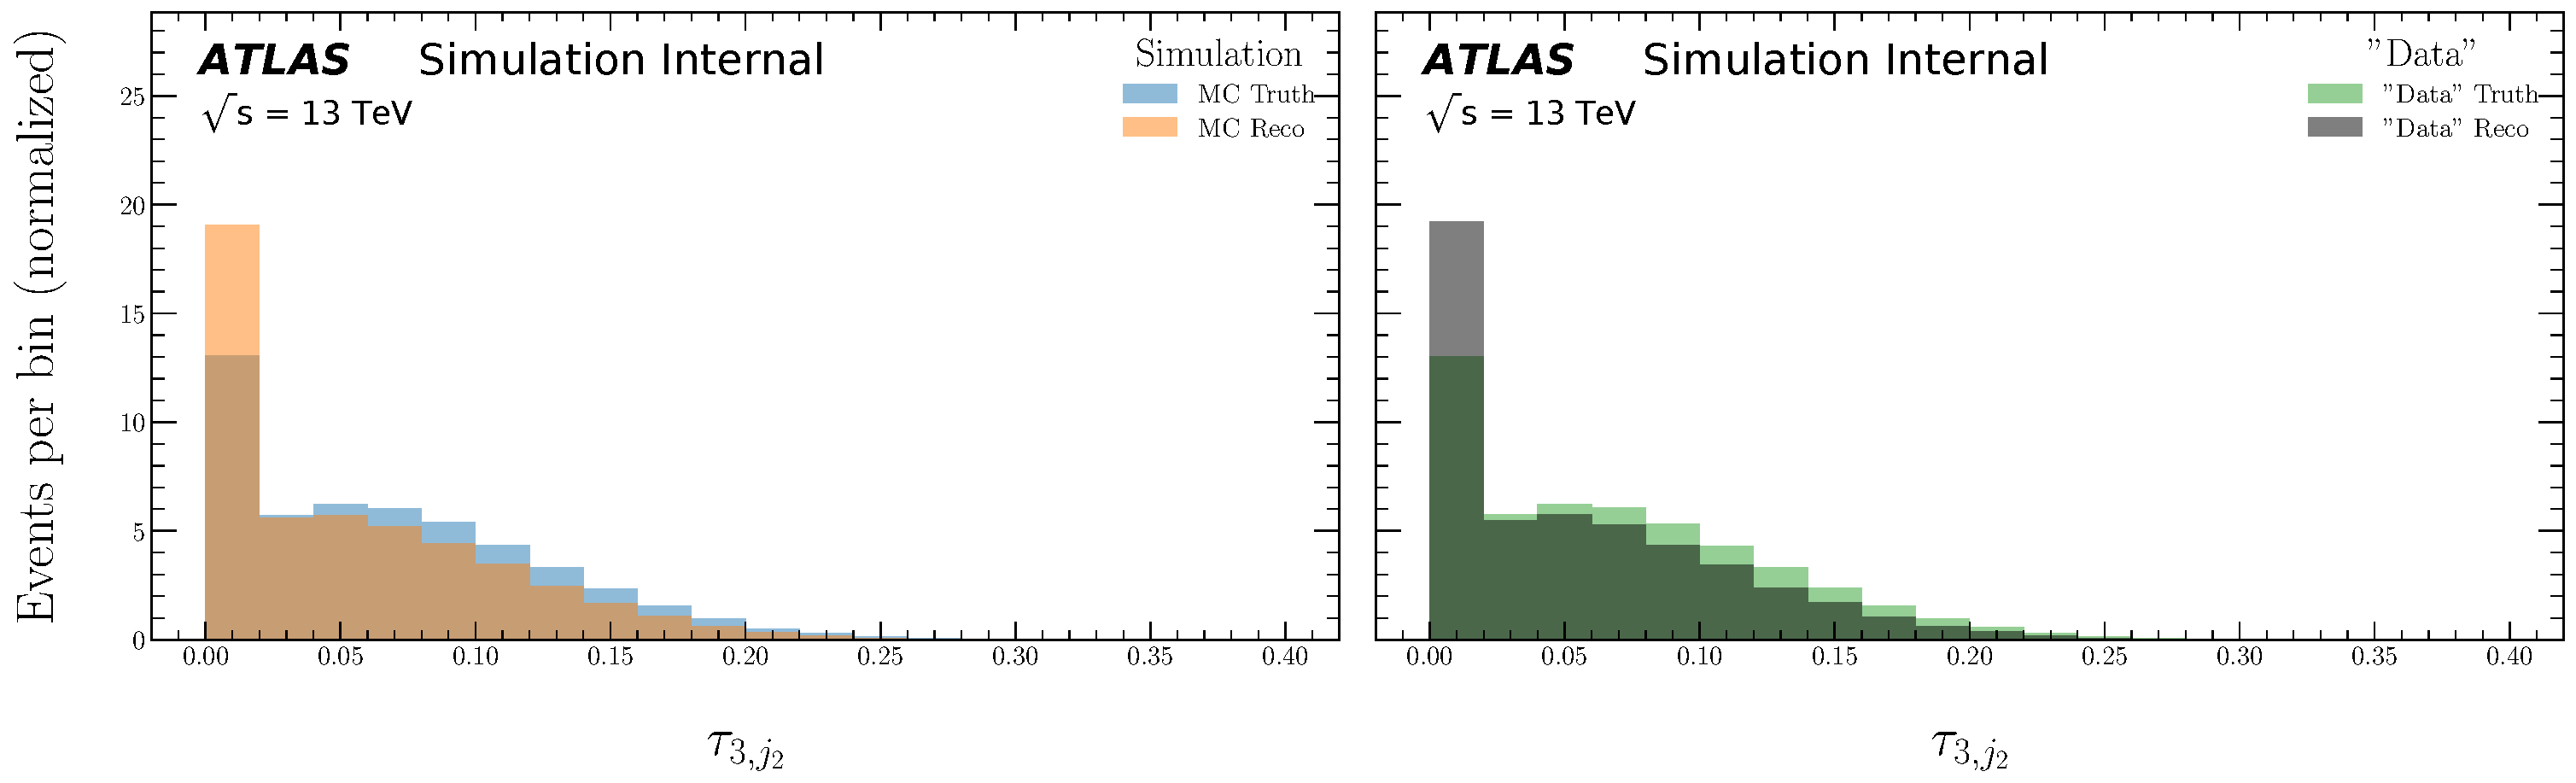
\includegraphics[width=0.89\textwidth]{figures/ATLASOmniFold-StressTest/ATLASOmniFold-TechnicalClosureTest/MultiFold/tau3_trackj2/ATLASOmniFold-TechnicalClosureTest-MultiFold-tau3_trackj2-Distributions.pdf}}\\
\subfloat[After 1 iteration]{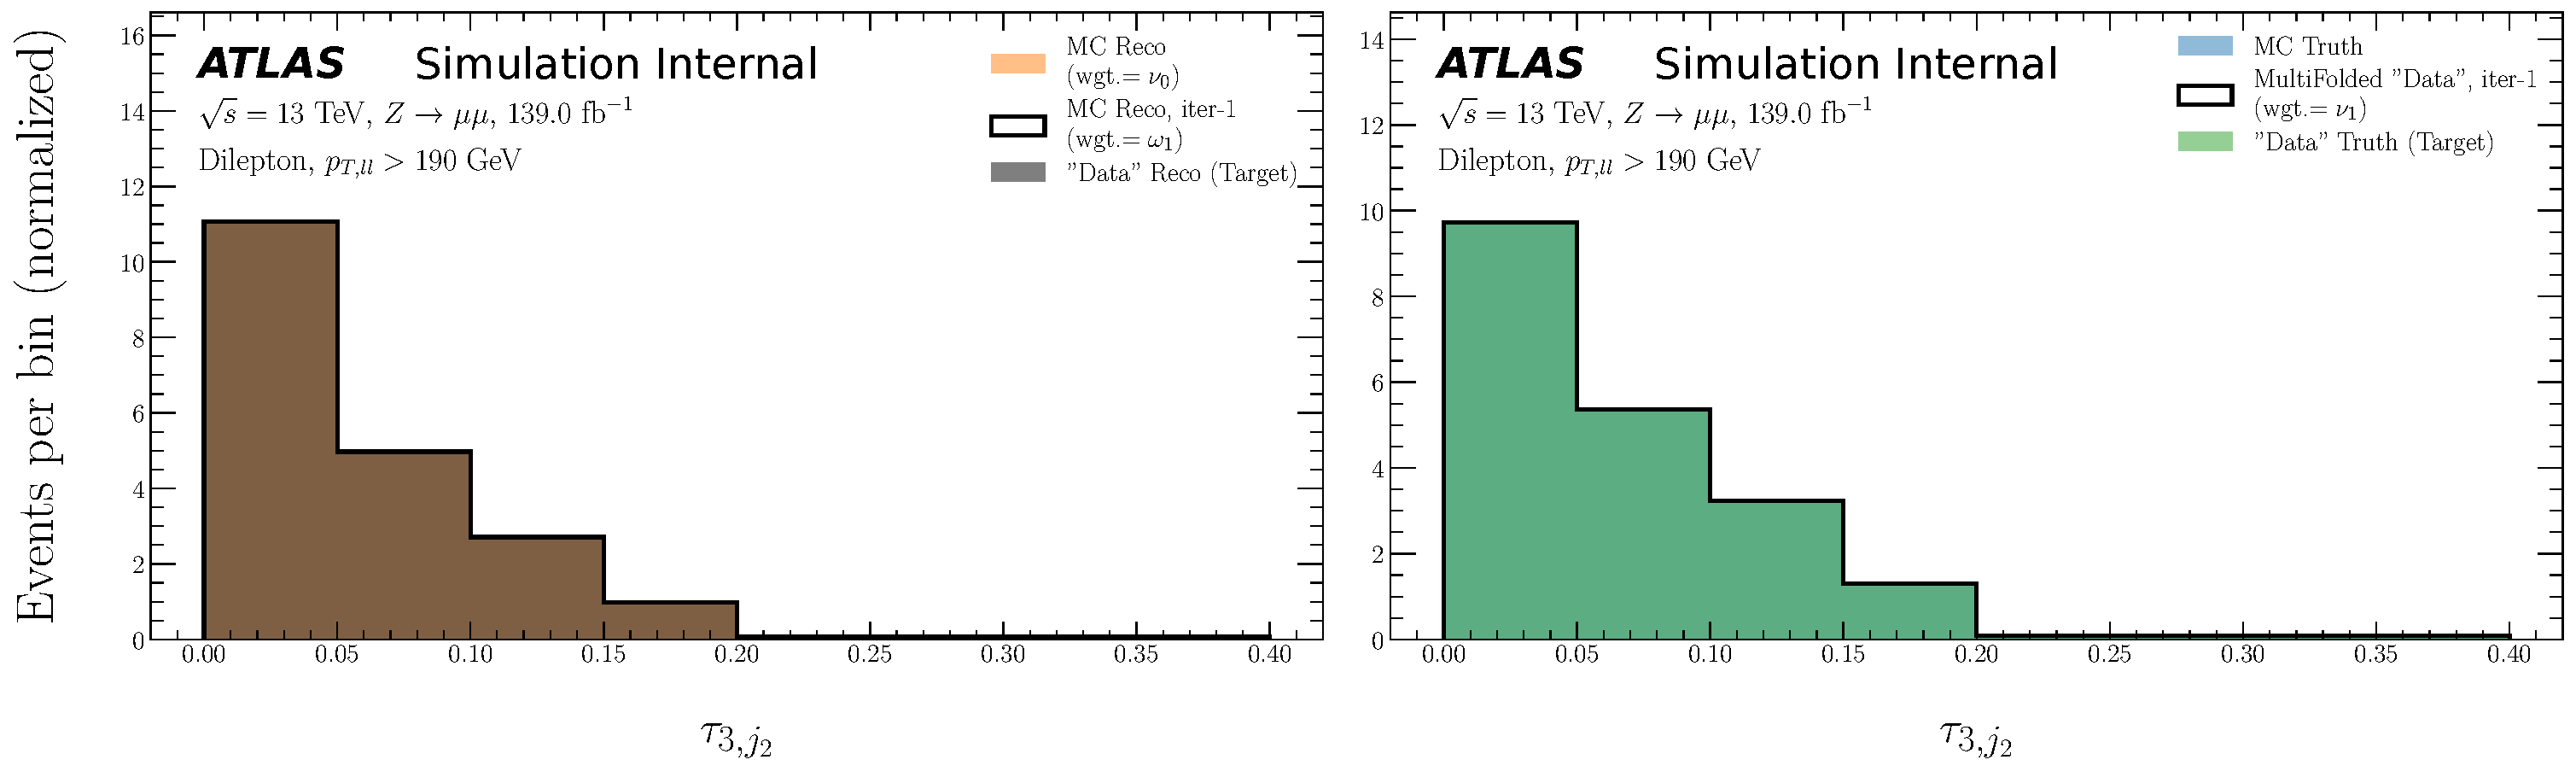
\includegraphics[width=0.95\textwidth]{figures/ATLASOmniFold-StressTest/ATLASOmniFold-TechnicalClosureTest/MultiFold/tau3_trackj2/ATLASOmniFold-TechnicalClosureTest-MultiFold-tau3_trackj2-Iteration01.pdf}}
\caption{A technical closure test for the $\tau_3$ of the subleading track jet using MultiFold (16 observables are simultaneously unfolded).  The top plot show the input histograms and the bottom plots are the results after one iteration of OmniFold.  By construction the top left and top right histograms are statistically identical.}
\label{fig:technicalclosureMulti:tau3_trackj2}
\end{figure}

\begin{figure}[h!]
\centering
\subfloat[Input histograms]{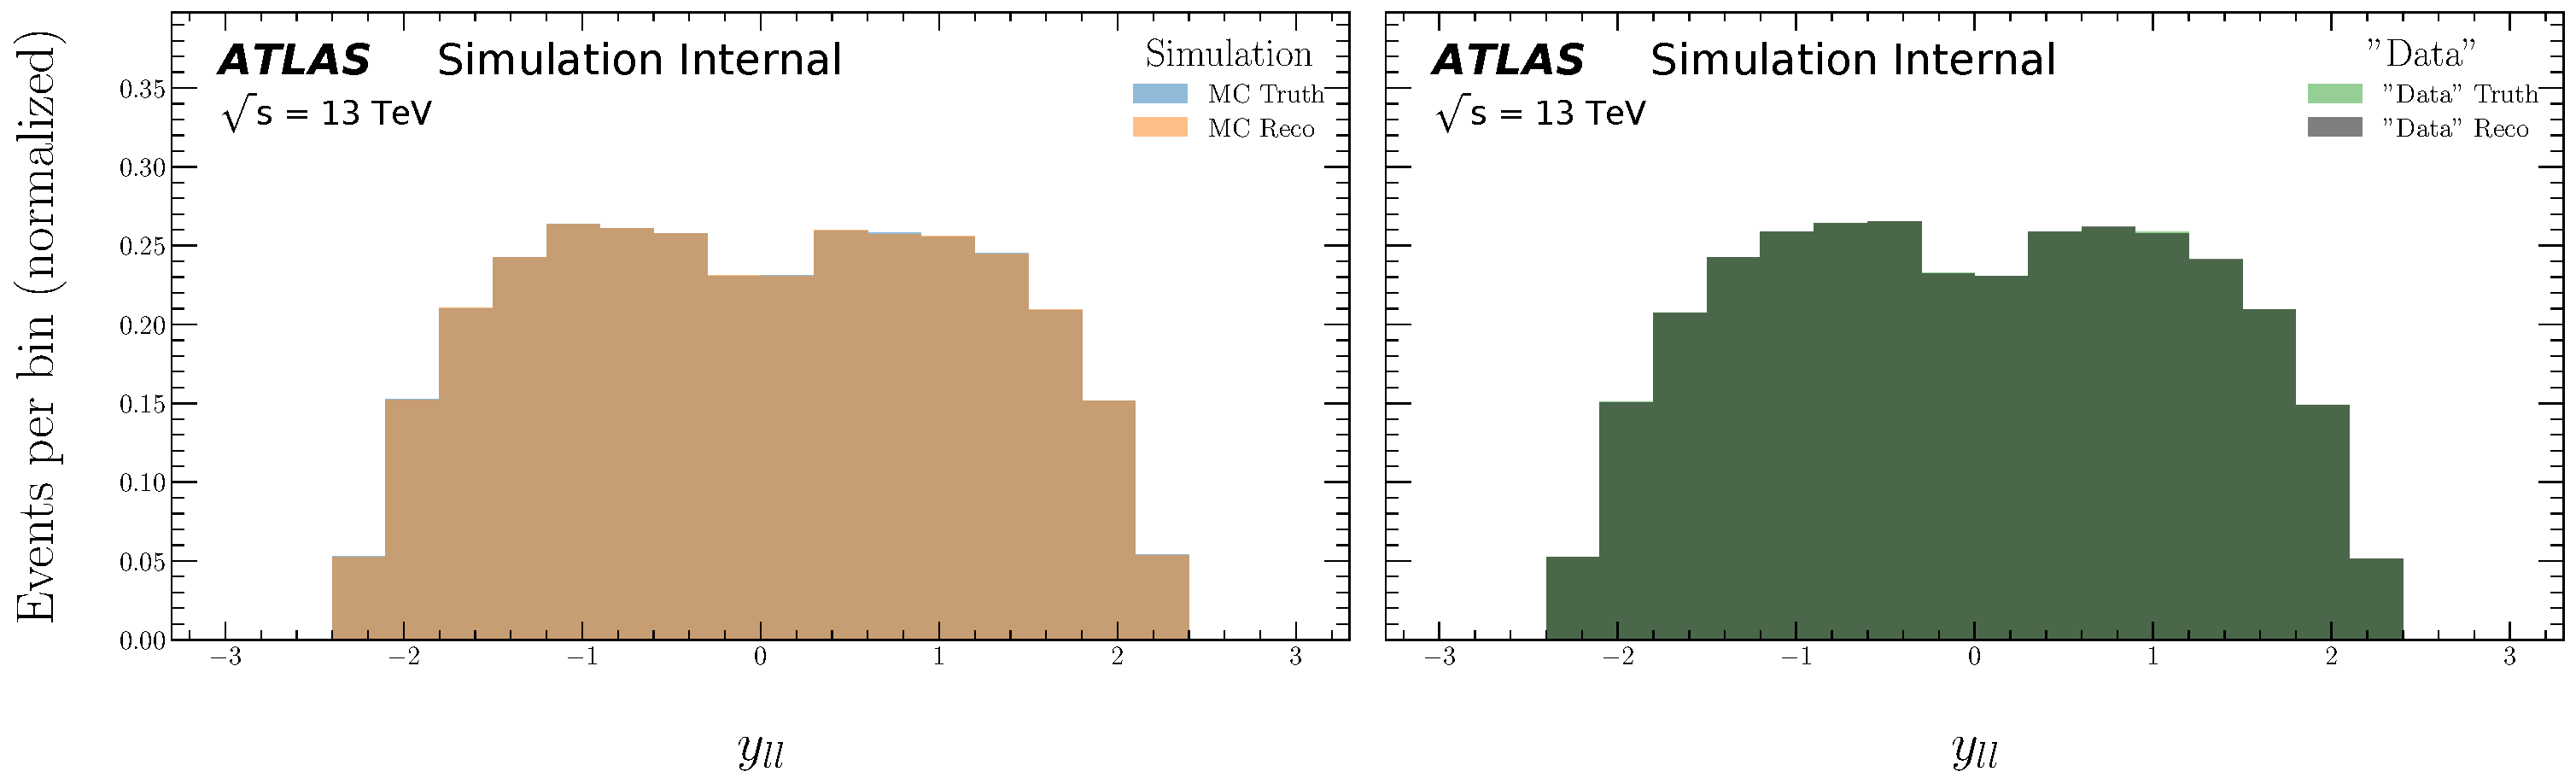
\includegraphics[width=0.89\textwidth]{figures/ATLASOmniFold-StressTest/ATLASOmniFold-TechnicalClosureTest/MultiFold/y_ll/ATLASOmniFold-TechnicalClosureTest-MultiFold-y_ll-Distributions.pdf}}\\
\subfloat[After 1 iteration]{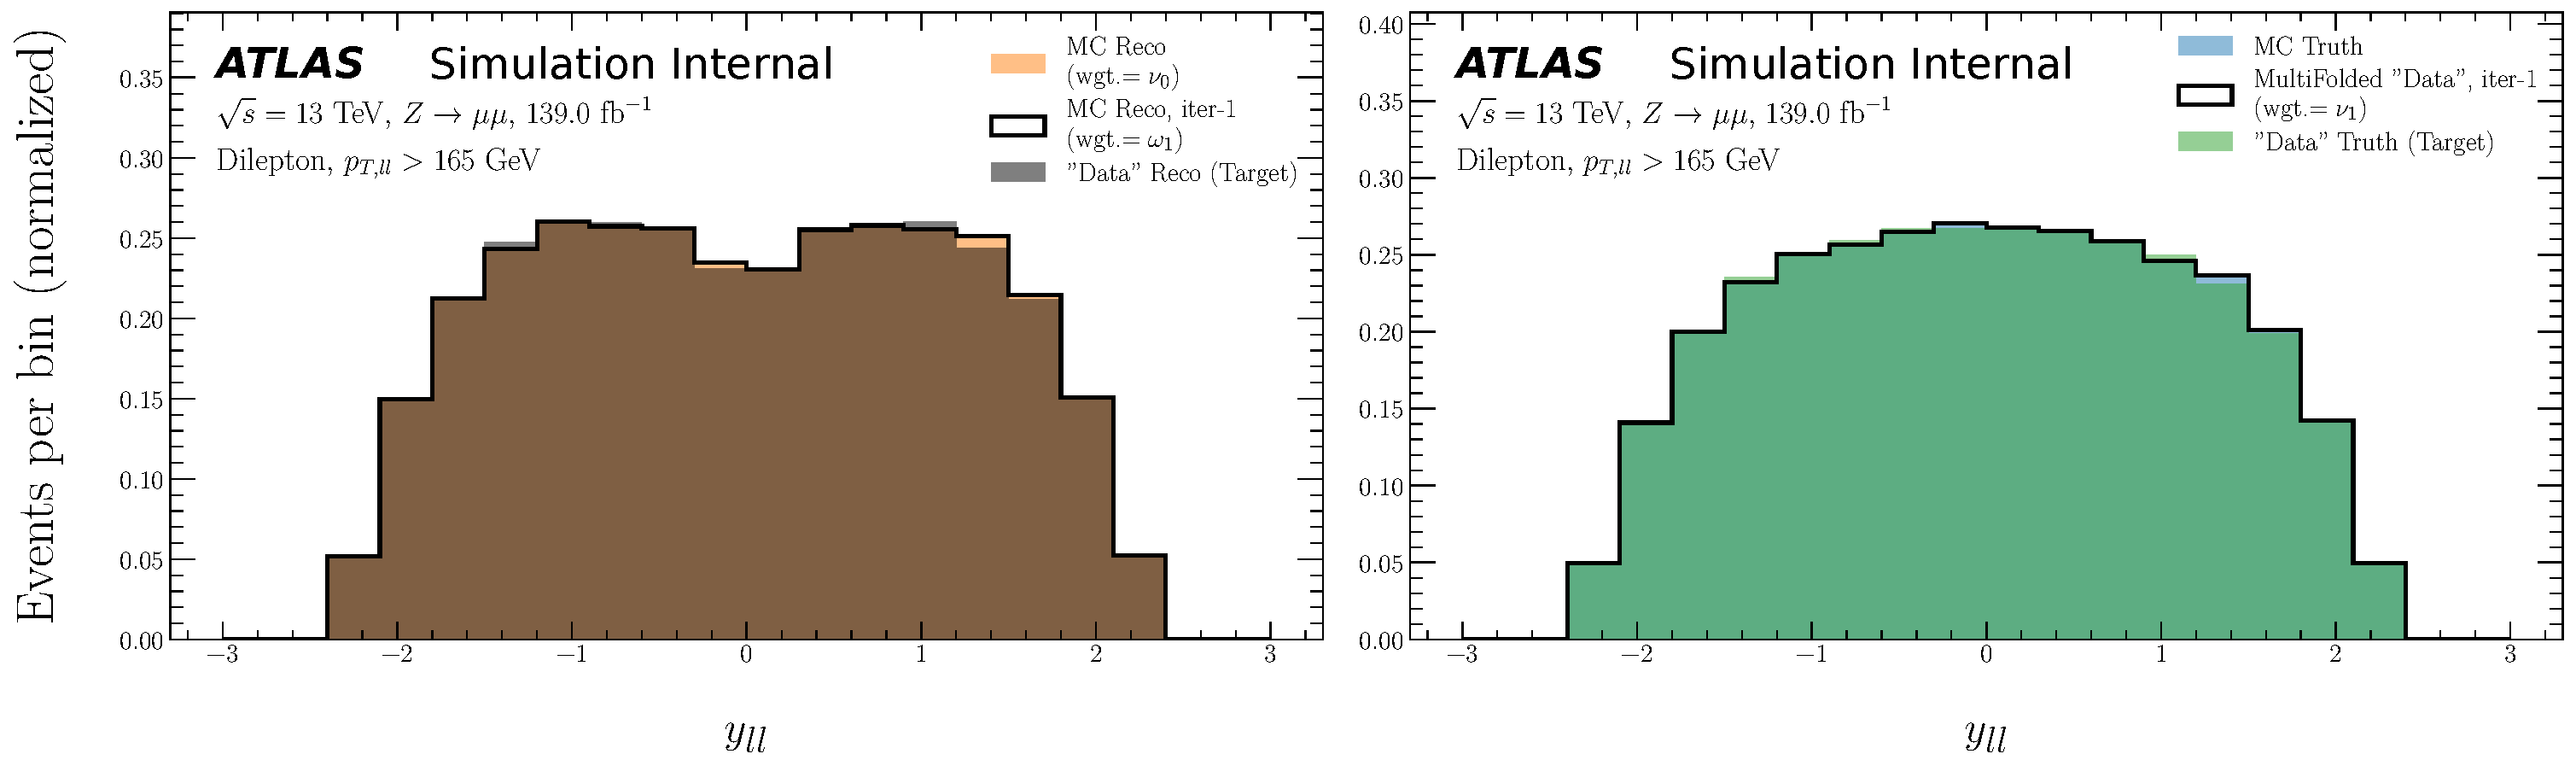
\includegraphics[width=0.95\textwidth]{figures/ATLASOmniFold-StressTest/ATLASOmniFold-TechnicalClosureTest/MultiFold/y_ll/ATLASOmniFold-TechnicalClosureTest-MultiFold-y_ll-Iteration01.pdf}}
\caption{A technical closure test for $y_{ll}$ using MultiFold (16 observables are simultaneously unfolded).  The top plot show the input histograms and the bottom plots are the results after one iteration of OmniFold.  By construction the top left and top right histograms are statistically identical.}
\label{fig:technicalclosureMulti:yll}
\end{figure}

\begin{figure}[h!]
\centering
\subfloat[Input histograms]{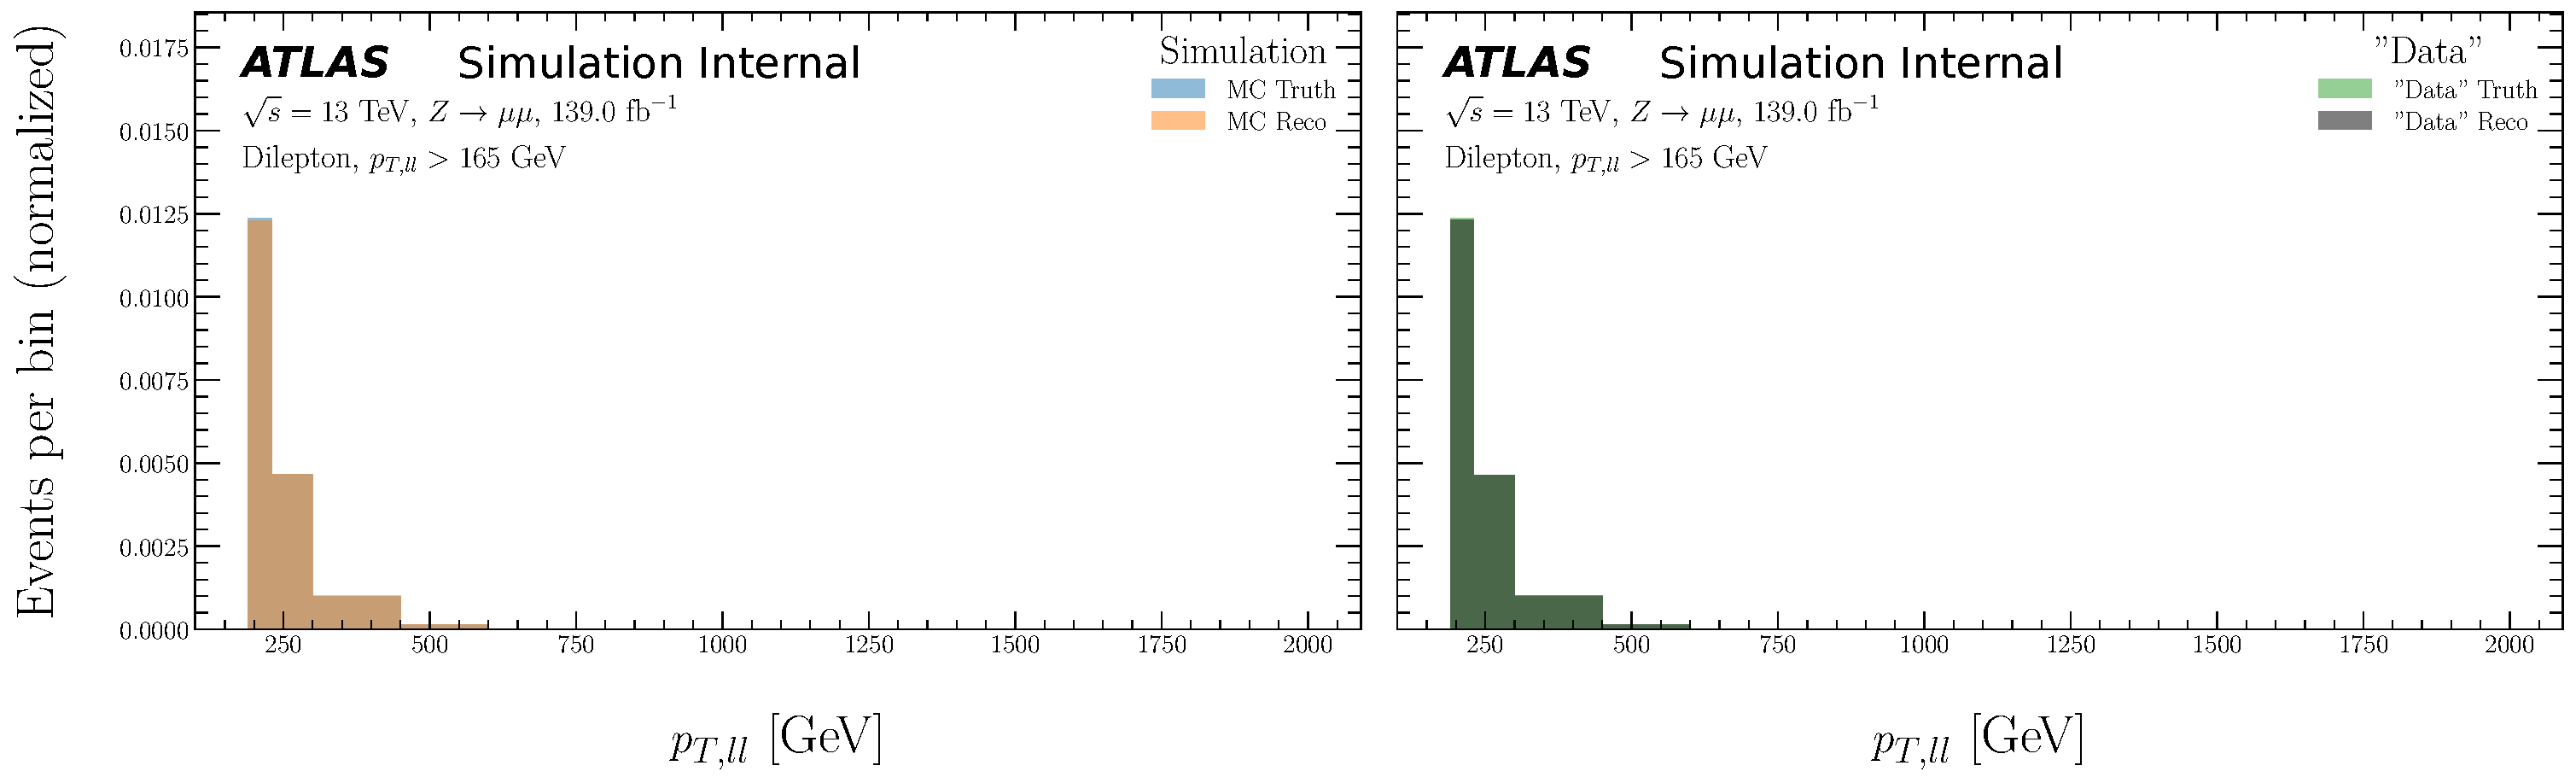
\includegraphics[width=0.89\textwidth]{figures/ATLASOmniFold-StressTest/ATLASOmniFold-TechnicalClosureTest/MultiFold/pT_ll/ATLASOmniFold-TechnicalClosureTest-MultiFold-pT_ll-Distributions.pdf}}\\
\subfloat[After 1 iteration]{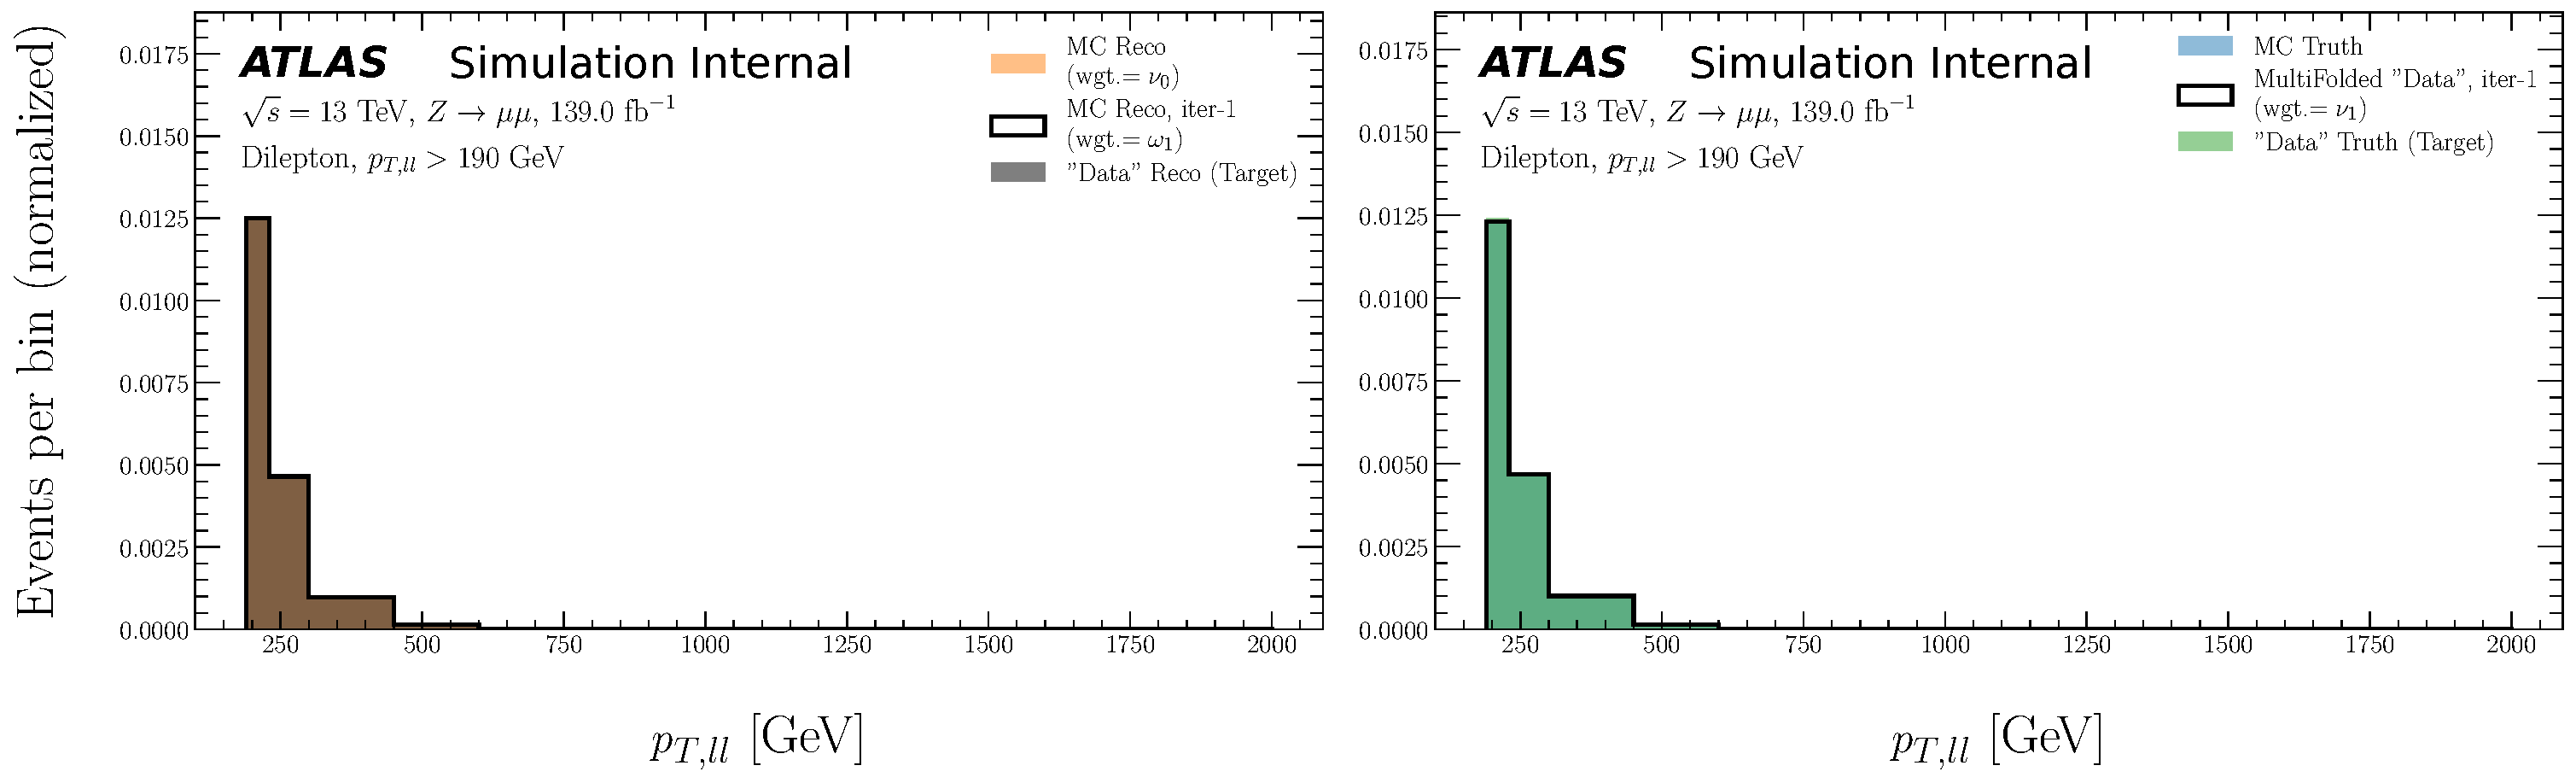
\includegraphics[width=0.95\textwidth]{figures/ATLASOmniFold-StressTest/ATLASOmniFold-TechnicalClosureTest/MultiFold/pT_ll/ATLASOmniFold-TechnicalClosureTest-MultiFold-pT_ll-Iteration01.pdf}}
\caption{A technical closure test for $p_{T,ll}$ using MultiFold (16 observables are simultaneously unfolded).  The top plot show the input histograms and the bottom plots are the results after one iteration of OmniFold.  By construction the top left and top right histograms are statistically identical.}
\label{fig:technicalclosureMulti:ptll}
\end{figure}
